% =========================================================
%  Chapter 10 — Photodetectors and Noise
%  Source: Dr. George's Lectures (Lecture 6)
%  Style: student-voice notes matching the personal style guide
% =========================================================

% ------------------------------------------------------------------
\section{The Other End of the Link}
% ------------------------------------------------------------------

Every photon that the laser diode generates, modulates, and launches into the fibre must eventually be converted back into an electrical signal. This conversion is the job of the photodetector — a reverse-biased semiconductor junction that absorbs incoming photons and generates a proportional electrical current. In a sense, the photodetector is the time-reverse of the LED: instead of injecting current to produce photons, we inject photons to produce current.

The physics that governs absorption is the same band-structure physics we have been building throughout this sequence. An electron in the valence band can absorb a photon and be excited to the conduction band, leaving a hole behind — exactly the reverse of the radiative recombination process. The condition is the same: the photon energy must satisfy $h\nu \geq E_g$ to bridge the bandgap. Below this threshold, the semiconductor is transparent; above it, absorption occurs.

% ------------------------------------------------------------------
\section{Optical Absorption in a Photodetector}
% ------------------------------------------------------------------

Consider a photodetector whose absorbing region has length $L$ and absorption coefficient $\alpha(\lambda)$ (the same parameter that appears in Beer's law for optical attenuation). Accounting for the surface reflectivity $R$ at the semiconductor-air interface, the optical power actually entering the device at the front surface ($z = 0$) after reflection loss is:
\begin{equation*}
    P(0) = P_0(1 - R)
\end{equation*}

As this power propagates through the absorbing layer, it decays exponentially according to Beer's law:
\begin{equation*}
    P(z) = P(0)\,e^{-\alpha z} = P_0(1 - R)\,e^{-\alpha z}
\end{equation*}

The power remaining and exiting after passing through the full active region of length $L$ is:
\begin{equation*}
    P(L) = P_0(1 - R)\,e^{-\alpha L}
\end{equation*}

The useful optical power absorbed inside the active region of the semiconductor is the difference between the power that enters at $z = 0$ and the power that escapes at $z = L$:
\begin{align*}
    P_\text{abs} &= P(0) - P(L) \\[6pt]
    &= P_0(1 - R) - P_0(1 - R)\,e^{-\alpha L} \\[6pt]
    &= P_0(1 - R)\left(1 - e^{-\alpha L}\right)
\end{align*}
This yields the final absorption result:
\begin{keyresult}
    \begin{equation}
        P_\text{abs} = P_0(1 - R)\!\left(1 - e^{-\alpha L}\right)
    \end{equation}
\end{keyresult}

\begin{figure}[H]
    \centering
    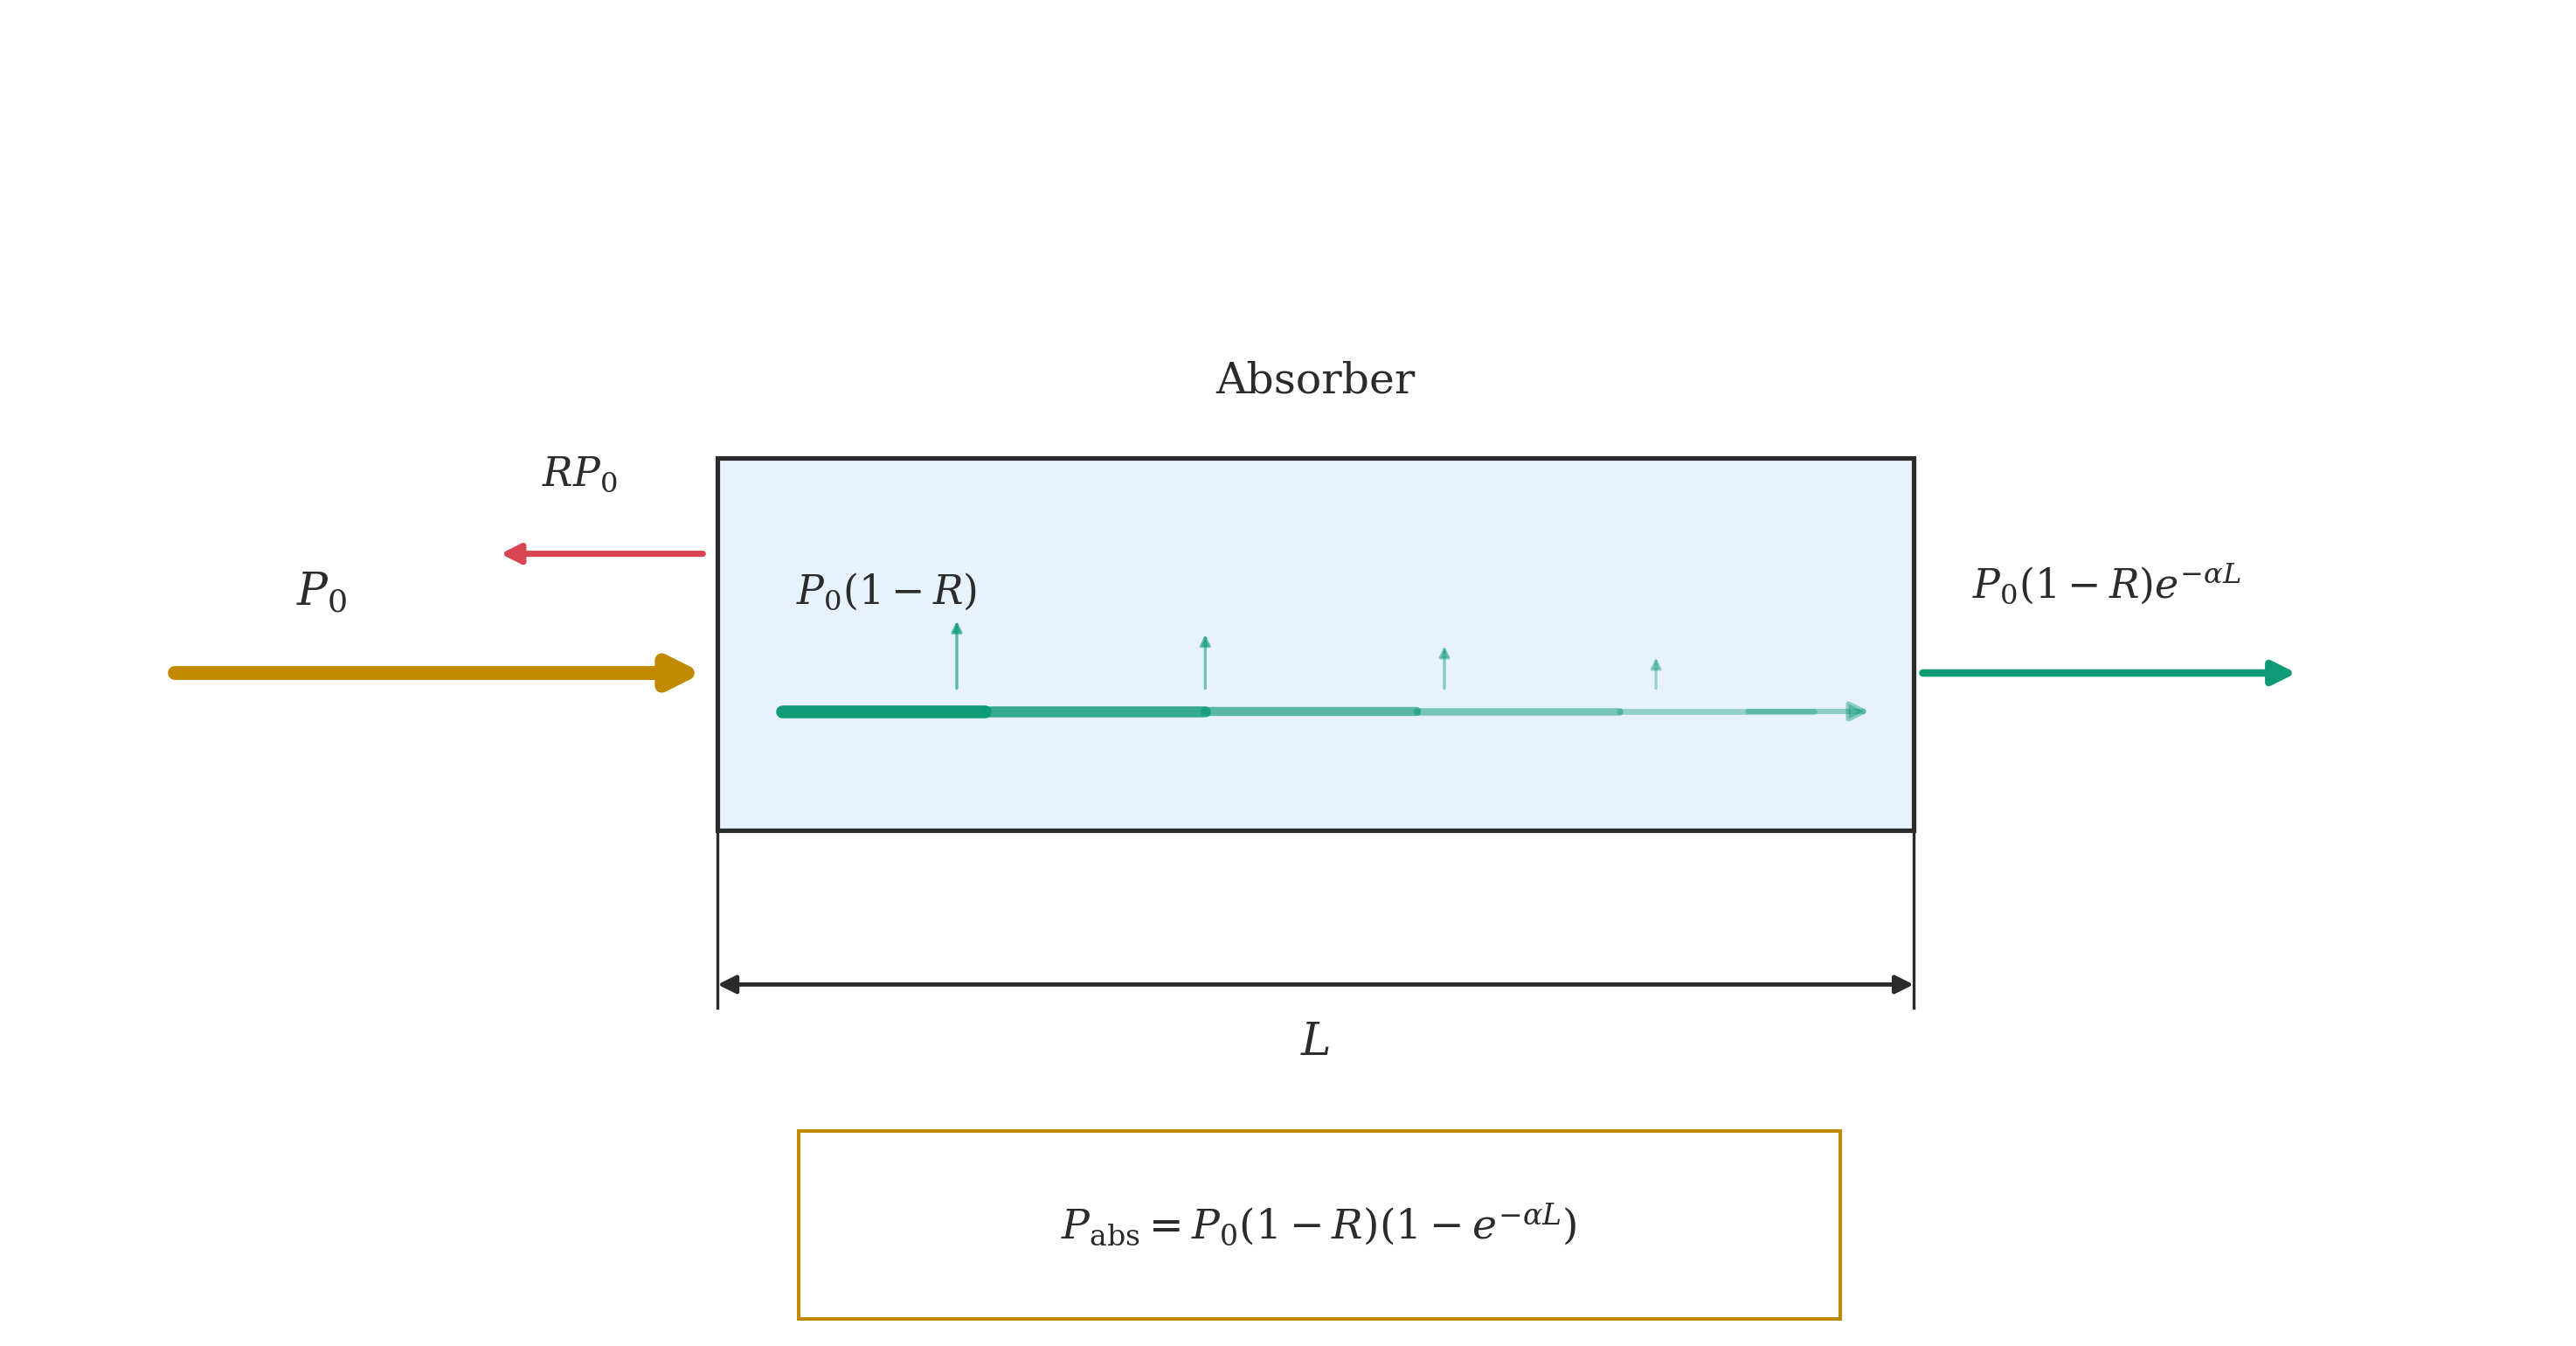
\includegraphics[width=0.6\textwidth]{Figures/Chapter 10/finite_absorbing_region_and_absorption_efficiency.jpg}
    \caption{Finite Absorbing Region and Absorption Efficiency}
    \label{fig:finite_absorbing_region_and_absorption_efficiency}
\end{figure}

This expression immediately tells us the two engineering levers for maximising absorption: reduce the surface reflectivity $R$ (using anti-reflection coatings) and increase $\alpha L$ (either by choosing a material with a high absorption coefficient at the operating wavelength, or by making the absorbing region thicker).

\begin{figure}[H]
    \centering
    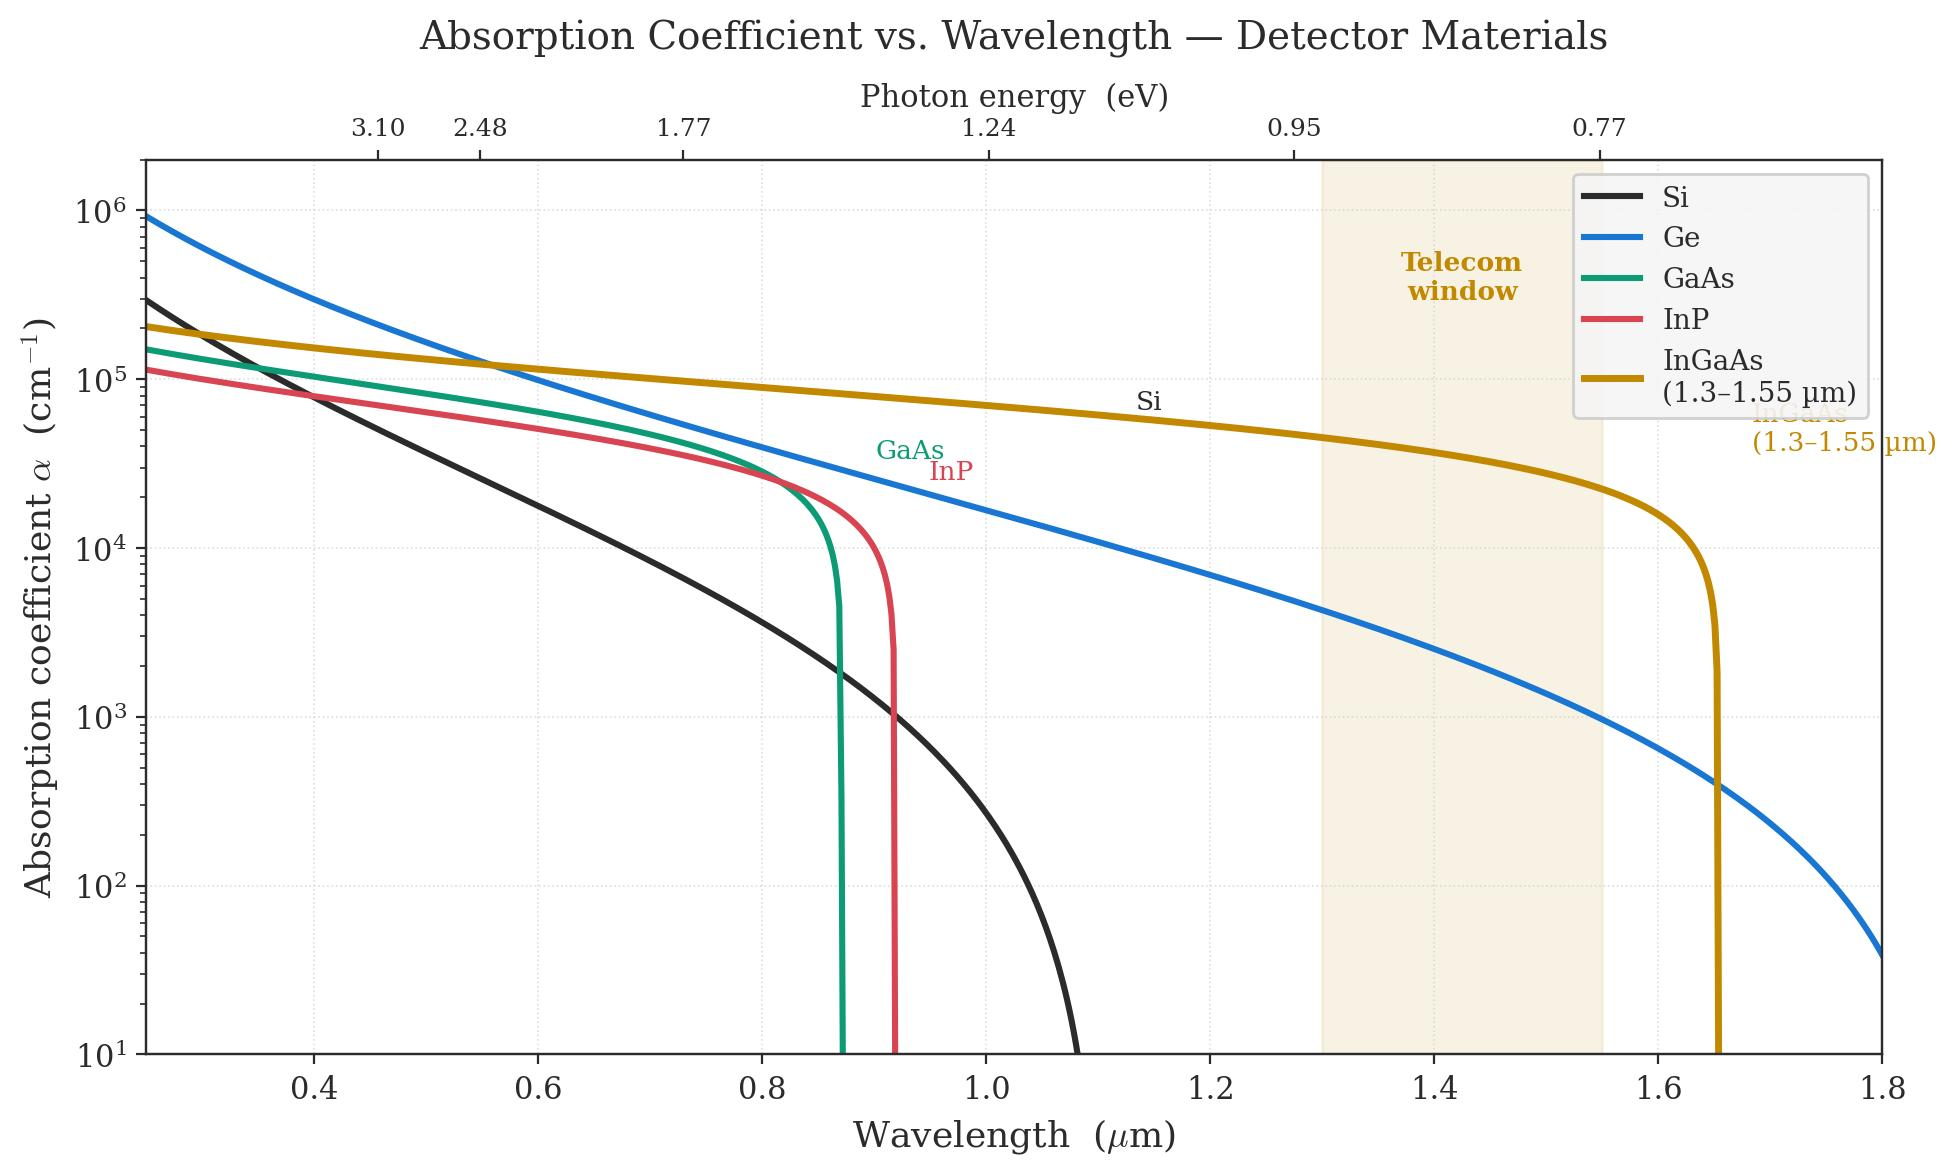
\includegraphics[width=0.6\textwidth]{Figures/Chapter 10/absorption_coefficient.jpg}
    \caption{Absorption Coefficient Versus Wavelength for Detector Materials}
    \label{fig:absorption_coefficient}
\end{figure}

% ------------------------------------------------------------------
\section{Quantum Efficiency and Responsivity}
% ------------------------------------------------------------------

\subsection{External Quantum Efficiency}

Not every absorbed photon successfully delivers an electron to the external circuit. Some photogenerated carriers recombine inside the device before being swept out by the electric field. The \textbf{external quantum efficiency} $\eta$ captures the end-to-end conversion from incident photons to collected electrons:
\begin{keyresult}
    \begin{equation}
        \eta = \frac{\text{electrons collected per second}}{\text{photons incident per second}} = \frac{I/e}{P_\text{opt}/(h\nu)}
    \end{equation}
\end{keyresult}

Breaking this down into its three contributing factors — reflection loss, incomplete absorption, and imperfect internal carrier collection — gives:
\begin{equation*}
    \eta = (1 - R)\!\left(1 - e^{-\alpha L}\right)\eta_\text{int}
\end{equation*}
where $\eta_\text{int}$ is the internal collection efficiency: the fraction of photogenerated carriers that are successfully swept to the contacts before recombining.

\subsection{Responsivity}

The \textbf{responsivity} $\mathcal{R}$ is the practical figure of merit that relates the measurable output current to the incident optical power:
\begin{equation*}
    \mathcal{R} \equiv \frac{I}{P_\text{opt}}
\end{equation*}

To express responsivity in terms of the external quantum efficiency $\eta$, we first isolate the output current $I$ from the definition of $\eta$:
\begin{equation*}
    \eta = \frac{I/e}{P_\text{opt}/(h\nu)} \implies I = e\eta\,\frac{P_\text{opt}}{h\nu}
\end{equation*}
Substituting this expression for $I$ into the responsivity definition gives:
\begin{equation*}
    \mathcal{R} = \frac{e\eta\,\dfrac{P_\text{opt}}{h\nu}}{P_\text{opt}} = \eta\,\frac{e}{h\nu}
\end{equation*}
To convert this frequency-scale responsivity to the wavelength scale, we substitute the dispersion relation for light in vacuum, $\nu = c/\lambda$, which yields:
\begin{keyresult}
    \begin{equation}
        \mathcal{R} = \eta\,\frac{e}{h\nu} = \eta\,\frac{e\lambda}{hc} \quad [\text{A/W}]
    \end{equation}
\end{keyresult}

\begin{figure}[H]
    \centering
    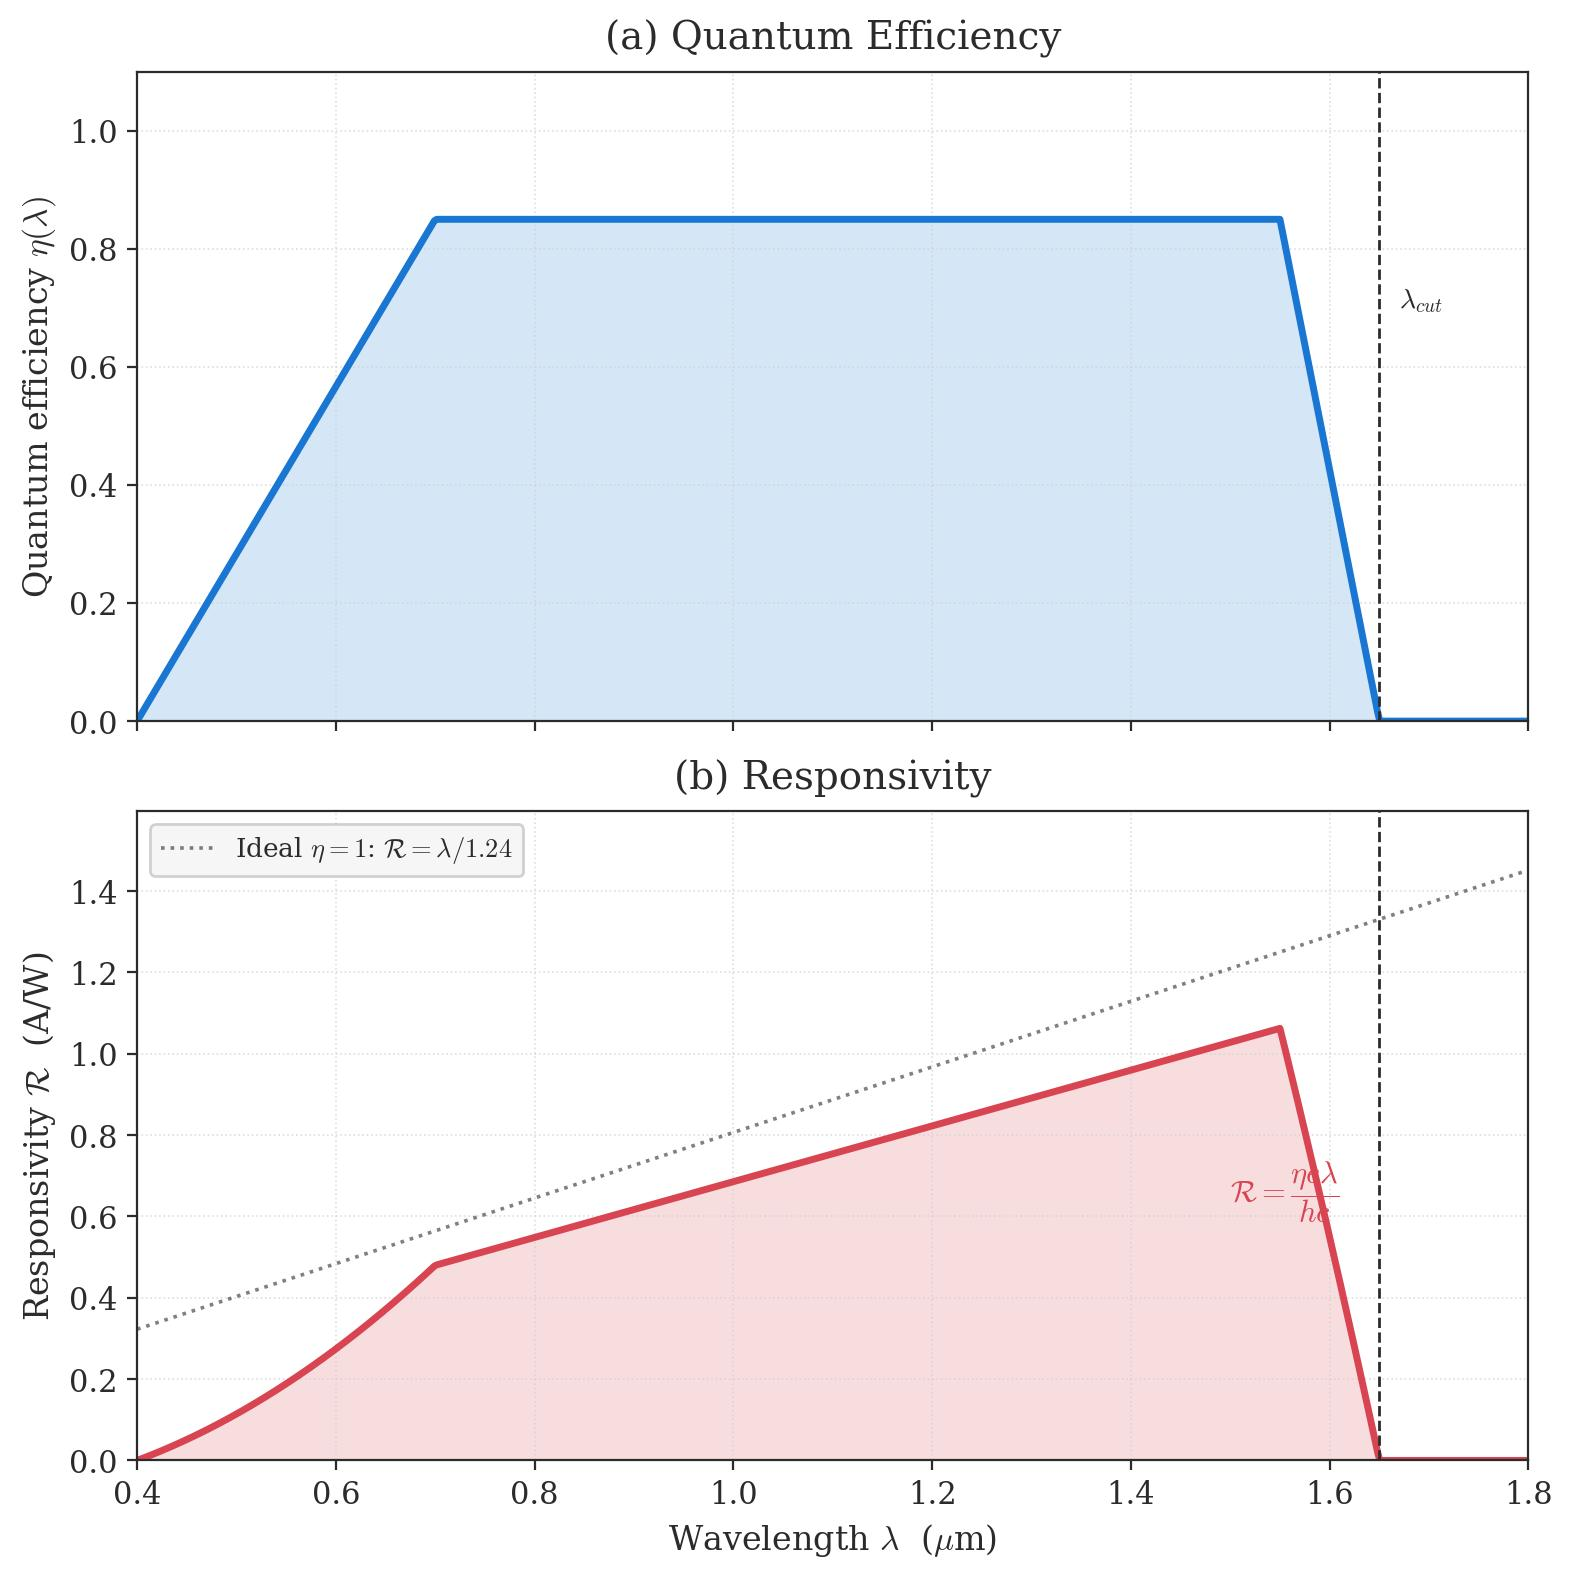
\includegraphics[width=0.7\textwidth]{Figures/Chapter 10/qe_and_responsivity.jpg}
    \caption{Quantum Efficiency and Responsivity Versus Wavelength}
    \label{fig:qe_and_responsivity}
\end{figure}

The wavelength dependence here is instructive: for fixed quantum efficiency, responsivity increases linearly with wavelength (longer wavelength photons carry less energy, so each watt of optical power represents more photons, generating more electrons). In practice, however, $\eta$ itself depends strongly on wavelength because the absorption coefficient $\alpha(\lambda)$ drops sharply below the bandgap — so there is always a long-wavelength cutoff at $\lambda_g = hc/E_g$ beyond which the material becomes transparent and the responsivity collapses to zero.

% ------------------------------------------------------------------
\section{PN Photodiode Operation}
% ------------------------------------------------------------------

A PN photodiode is operated under reverse bias, which establishes a strong electric field across the depletion region. When a photon is absorbed anywhere in the device, it creates an electron-hole pair. What happens next depends on exactly where that pair was created.

\begin{figure}[H]
    \centering
    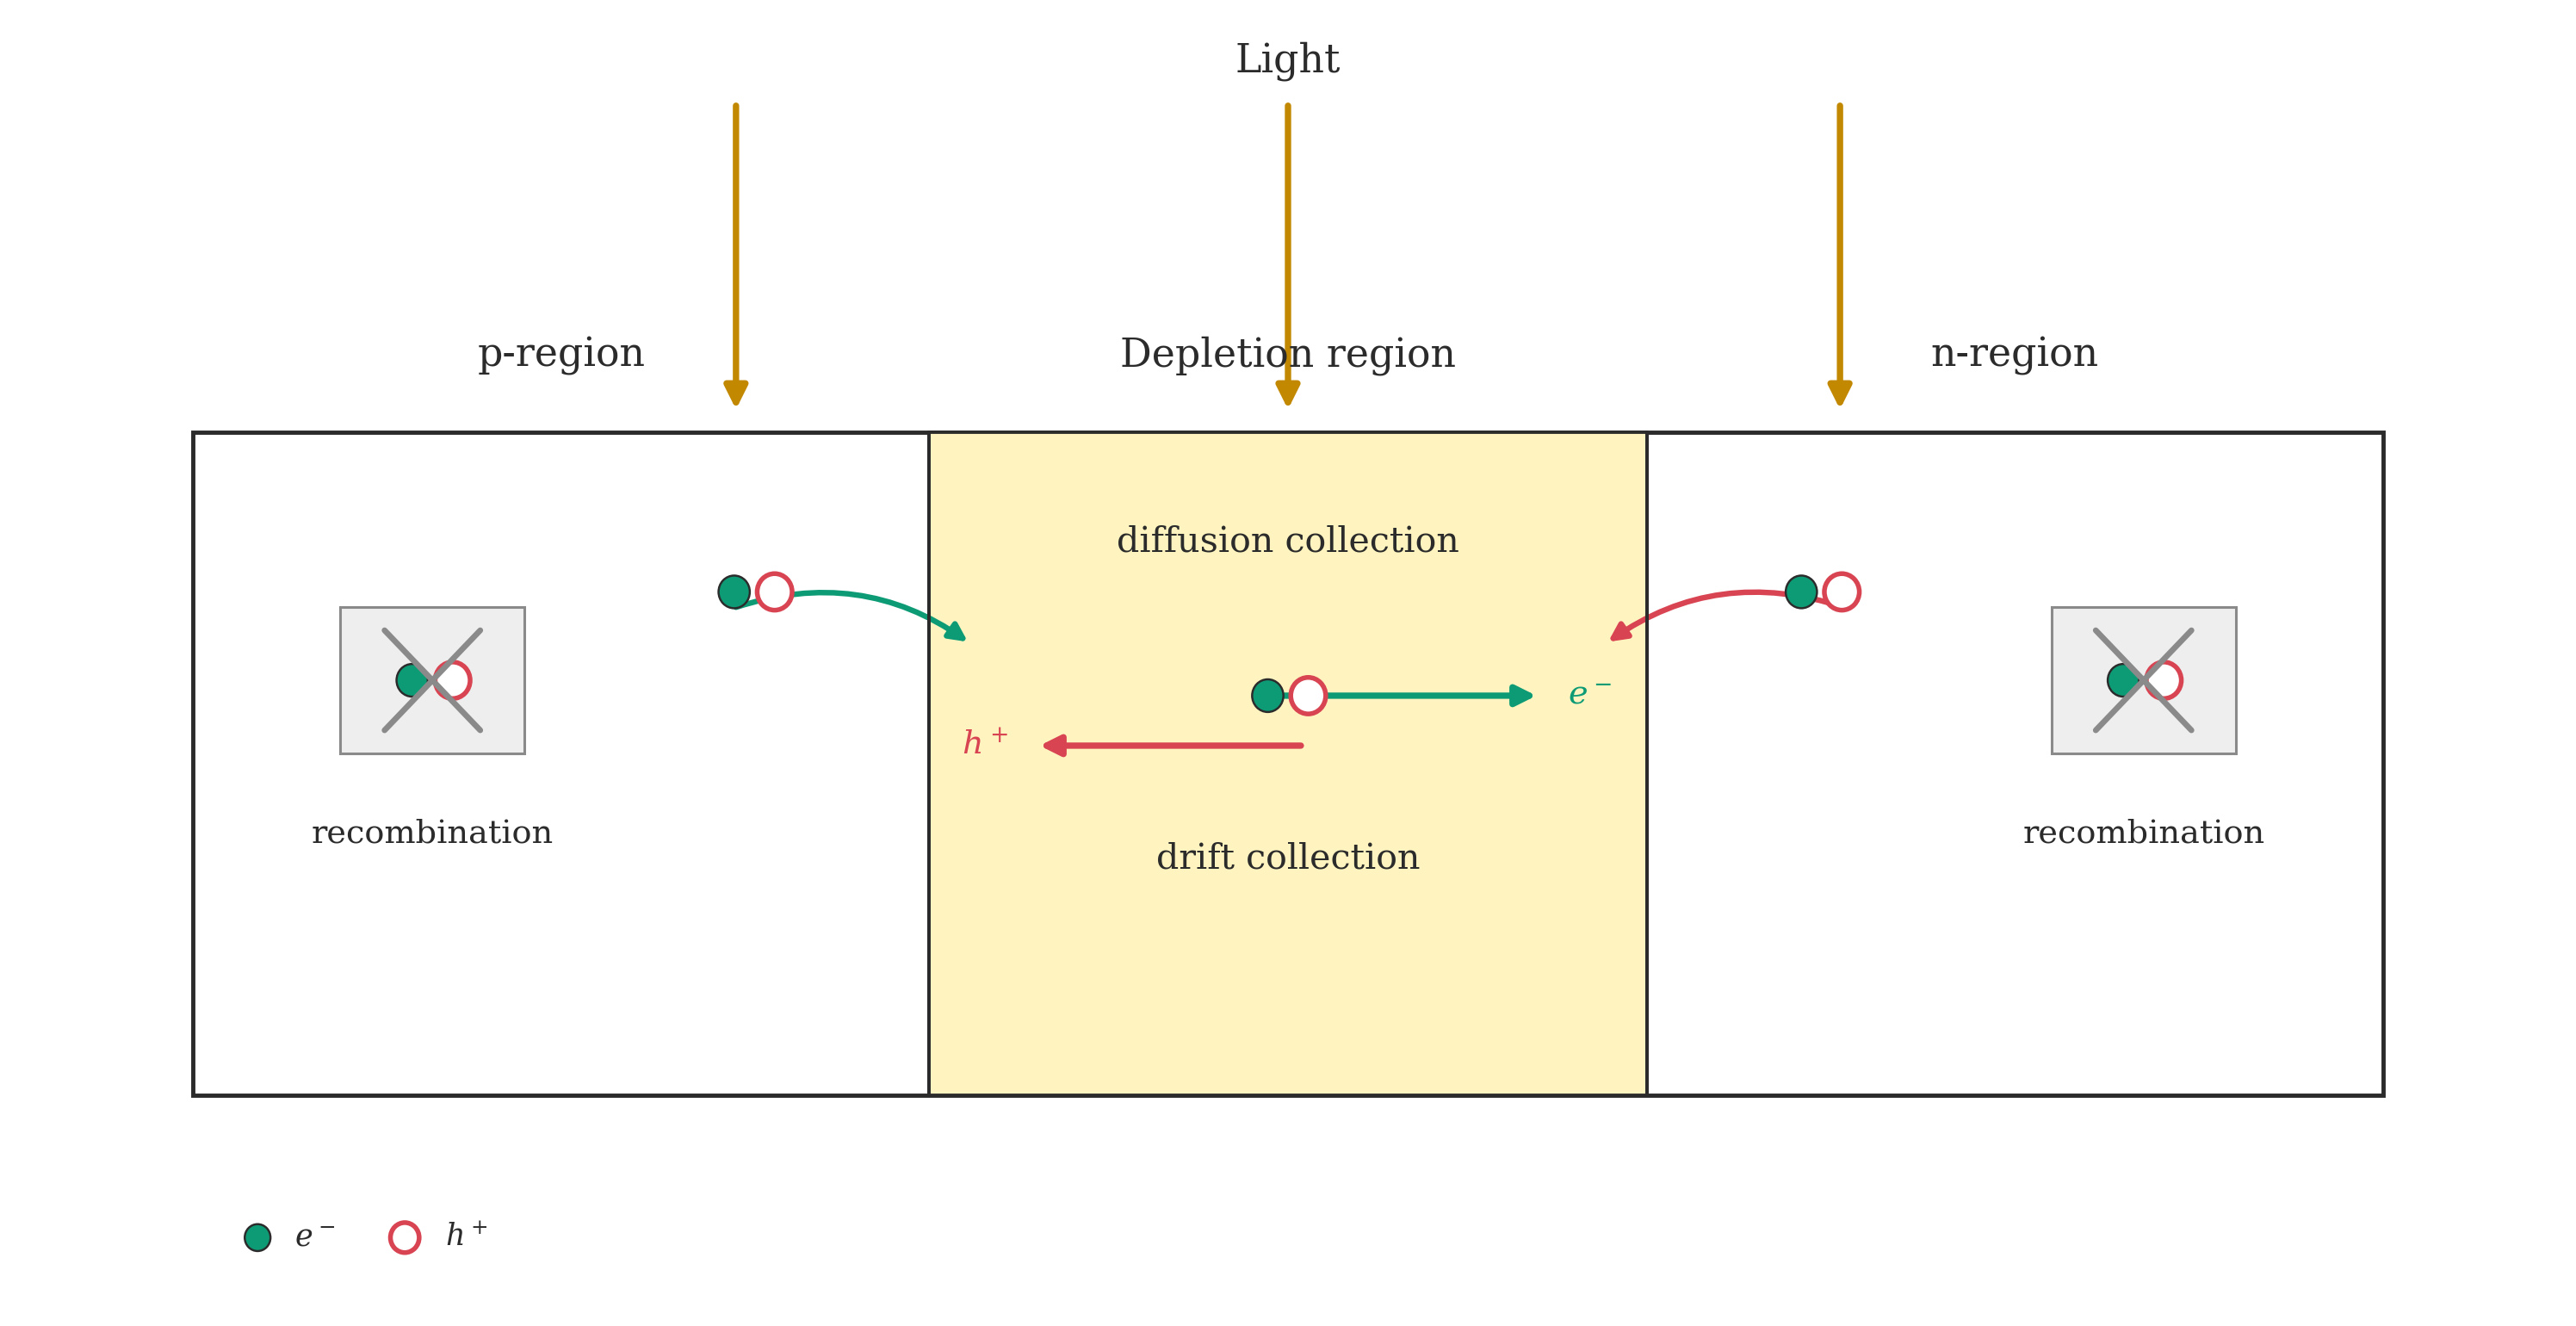
\includegraphics[width=0.6\textwidth]{Figures/Chapter 10/pn_photodiode_collection_regions.jpg}
    \caption{PN Photodiode Collection Regions}
    \label{fig:pn_photodiode_collection_regions}
\end{figure}

\subsection{Drift Collection from the Depletion Region}

Carriers generated \emph{inside} the depletion region immediately experience the strong built-in electric field, which rapidly sweeps electrons toward the n-side and holes toward the p-side. This drift process is fast — limited only by the carrier saturation velocity $v_d \approx 10^7\,\text{cm/s}$ in most III-V semiconductors — and is the dominant, efficient collection mechanism.

\begin{figure}[H]
    \centering
    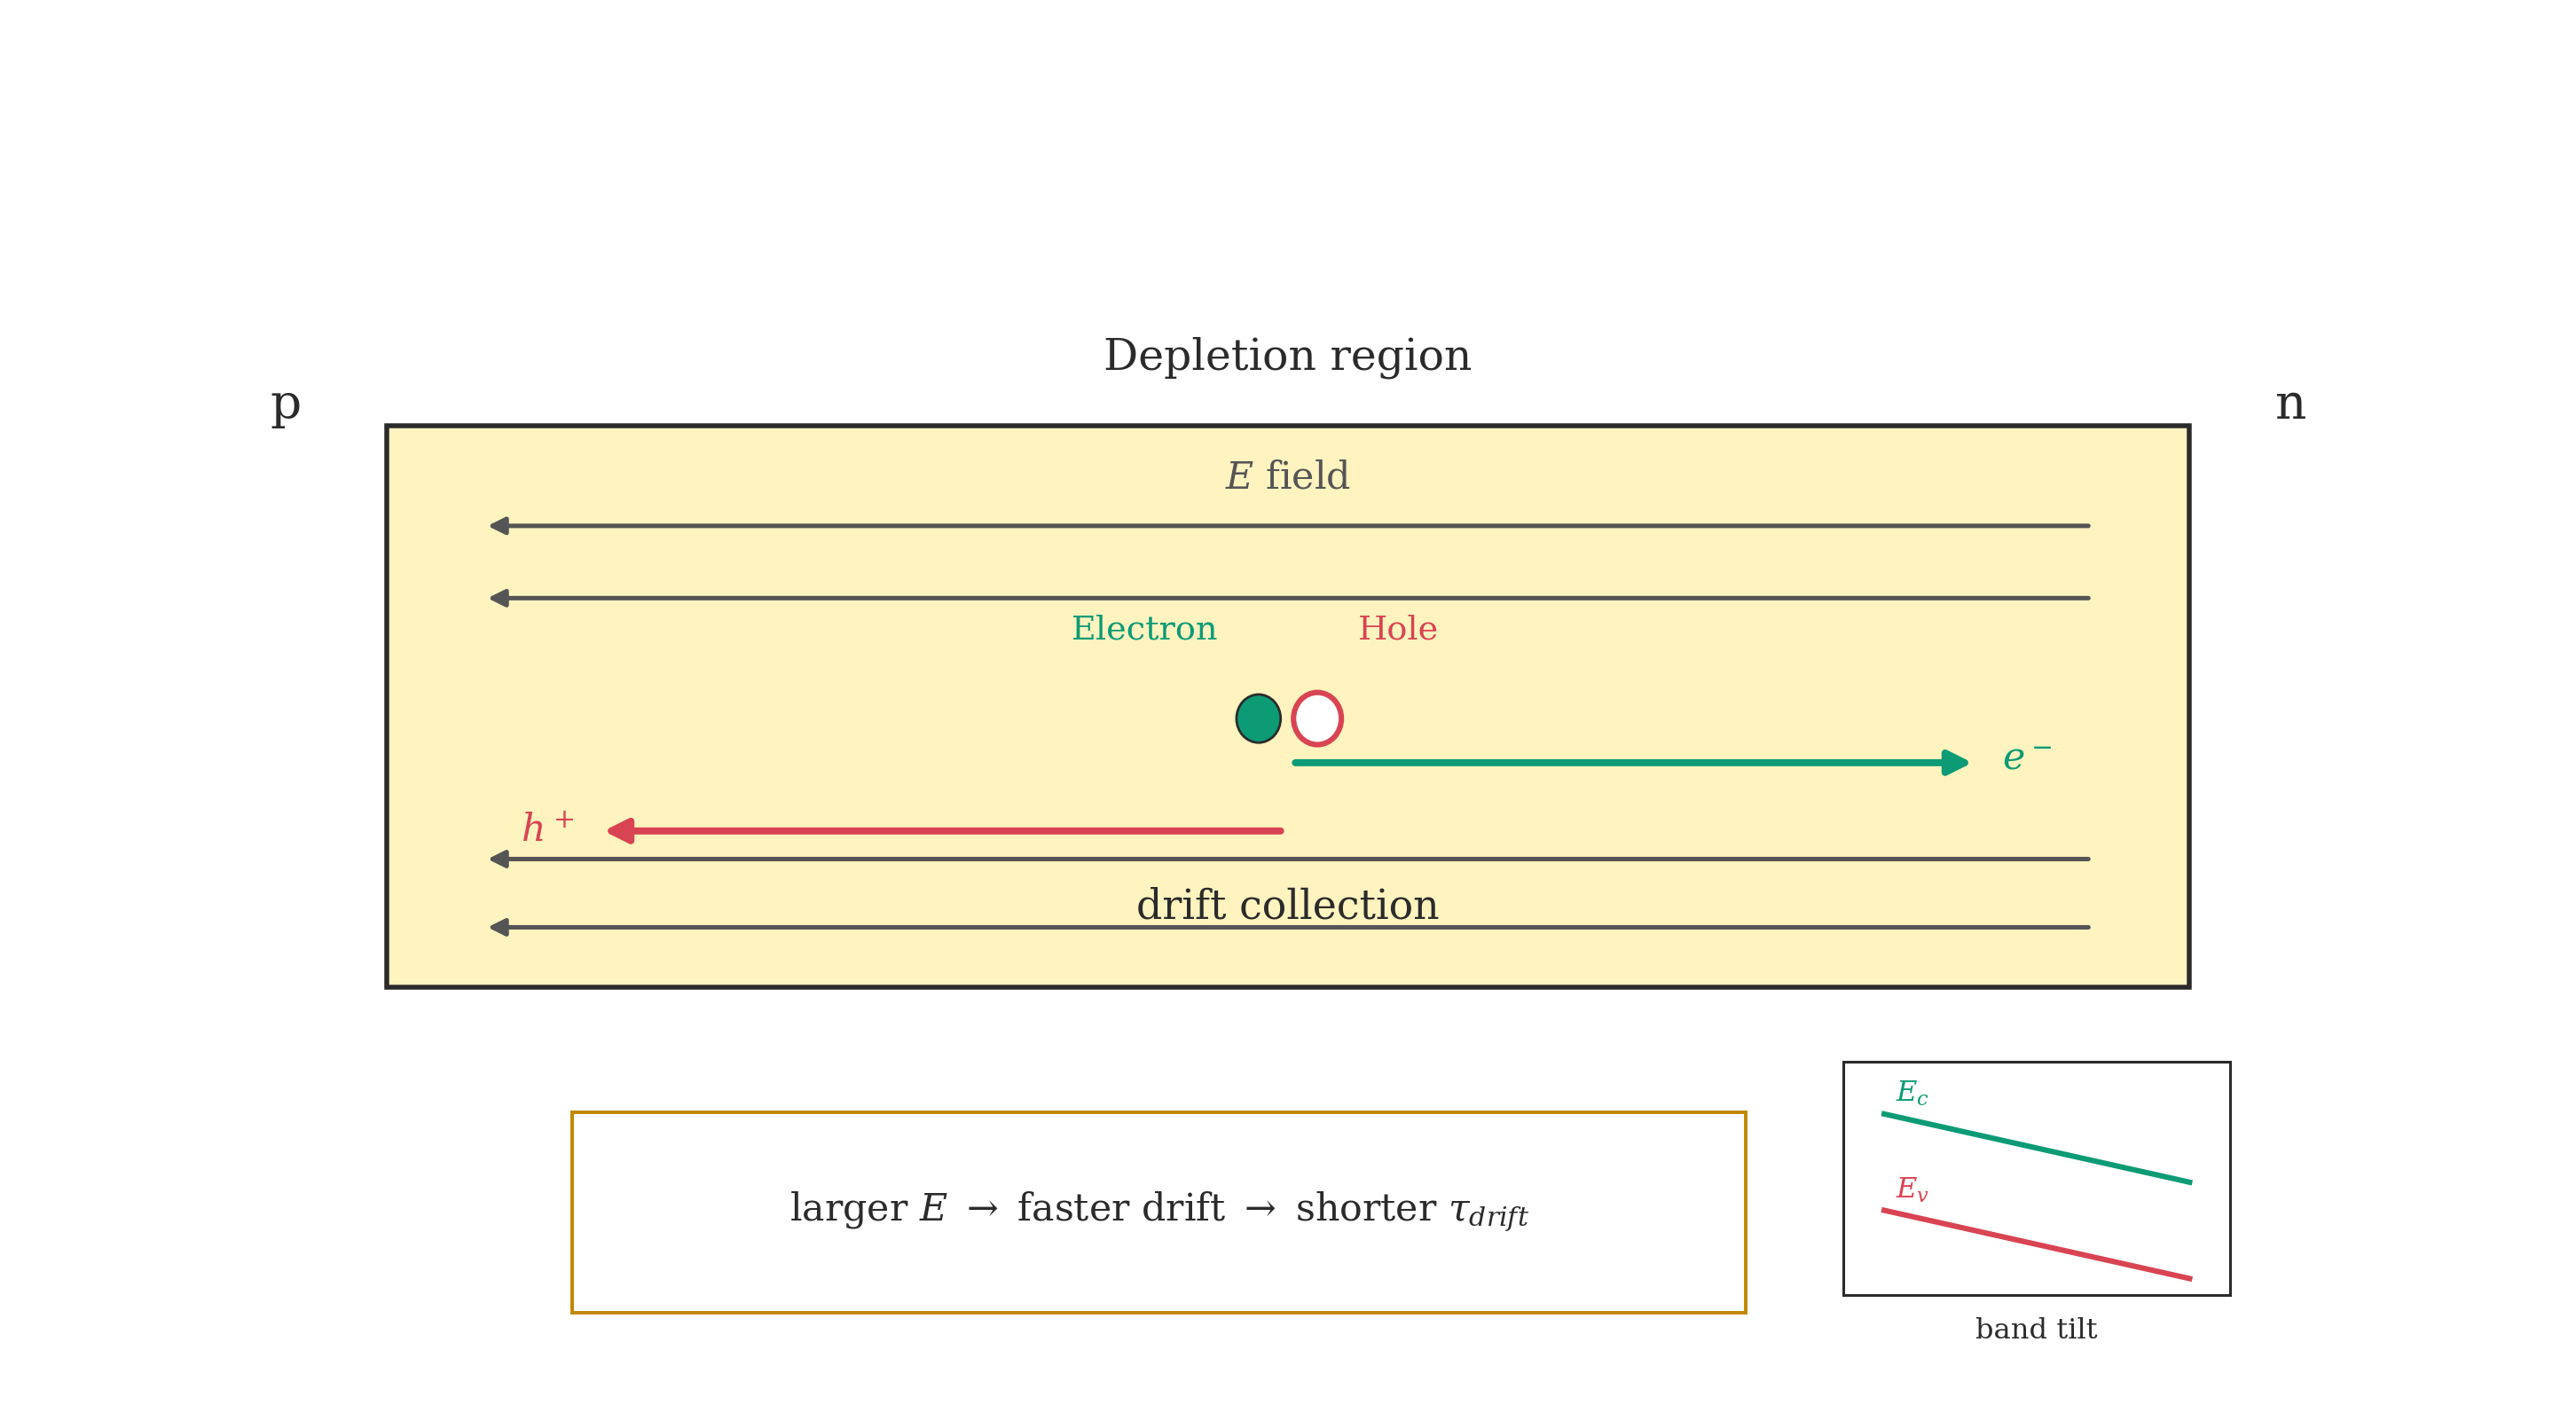
\includegraphics[width=0.6\textwidth]{Figures/Chapter 10/driftdominated_collection_in_the_depletion_region.jpg}
    \caption{Drift-Dominated Collection in the Depletion Region}
    \label{fig:driftdominated_collection_in_the_depletion_region}
\end{figure}

\subsection{Diffusion Collection from the Neutral Regions}

Carriers generated in the \emph{neutral} p or n regions outside the depletion layer do not immediately feel the field. They must first diffuse to the depletion edge before they can be swept across. If a carrier is generated close enough to the depletion edge (within roughly one diffusion length $L_e$ or $L_h$), it has a good chance of reaching the edge before recombining and contributes to the photocurrent. Carriers generated farther away are lost by recombination and do not contribute — they represent wasted absorption.

\begin{figure}[H]
    \centering
    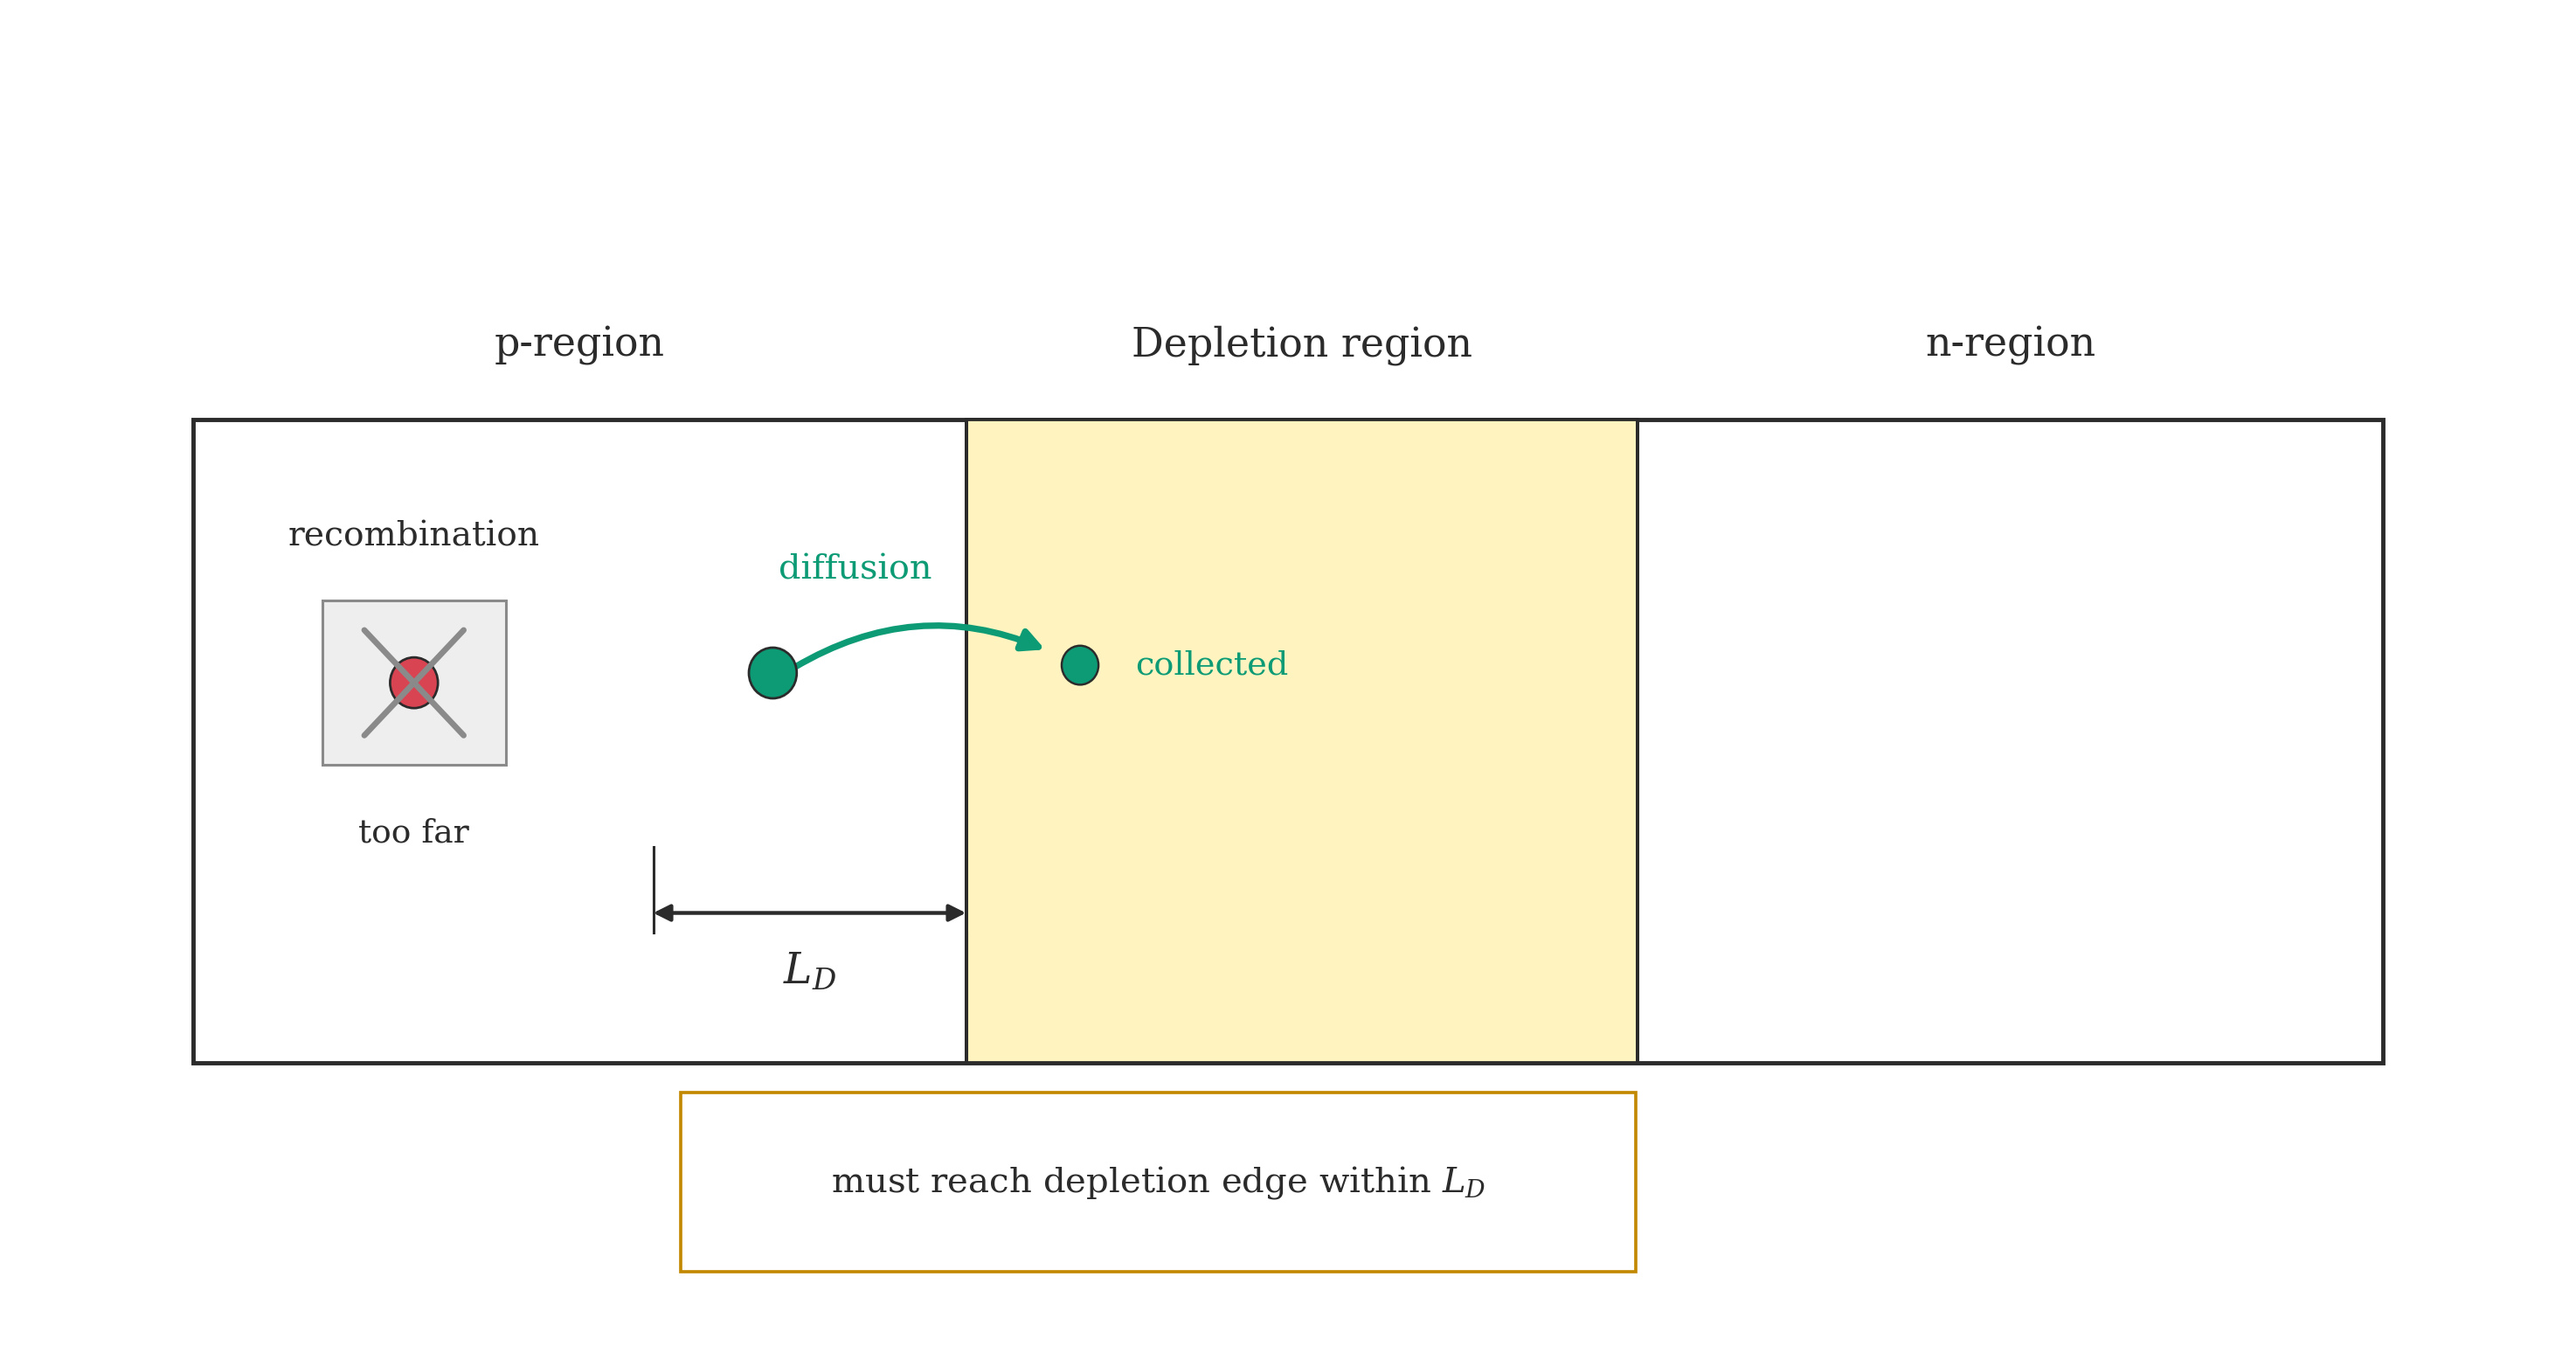
\includegraphics[width=0.6\textwidth]{Figures/Chapter 10/diffusion_collection_from_the_neutral_region.jpg}
    \caption{Diffusion Collection from the Neutral Region}
    \label{fig:diffusion_collection_from_the_neutral_region}
\end{figure}

\subsection{Wavelength Dependence of Collection}

The absorption depth at which photons are absorbed scales as $1/\alpha$: short-wavelength (high-energy) photons are absorbed very close to the surface (small $1/\alpha$), while long-wavelength photons penetrate deeper before being absorbed. This wavelength dependence creates a non-trivial spectral response:

At short wavelengths, most absorption happens near the illuminated surface — often within the neutral region — where collection is diffusion-limited and therefore less efficient. At the optimal wavelength, absorption is centred in the depletion region and $\eta$ is maximised. At wavelengths approaching $\lambda_g$, the absorption coefficient drops and $\alpha L \ll 1$: the device becomes transparent and $\eta \to 0$. The responsivity spectrum therefore peaks at an intermediate wavelength and rolls off on both sides.

\subsection{Rigorous Quantum Efficiency Model: The Dead Layer}

Let us build a strict mathematical model of optical absorption. A practical photodiode features an inactive, heavily doped top contact layer of thickness $x_0$ before the depletion region of width $W$. Because the doping in $x_0$ is extremely heavy and it sits right at the surface, the carrier lifetime is vanishingly short due to rapid surface recombination. Any photons absorbed in this layer are instantly lost. We call this the \textbf{dead layer}.

We start with the incident optical power $P_{\text{inc}}$ shining on the top surface. After reflection $R$, the power that enters the semiconductor is $P(0) = P_{\text{inc}}(1 - R)$.

As this light propagates through the dead layer, it decays exponentially. The power that survives and successfully reaches the edge of the active depletion region ($x = x_0$) is:
\begin{equation*}
    P(x_0) = P_{\text{inc}}(1 - R)\,e^{-\alpha x_0}
\end{equation*}

Once inside the depletion region (spanning from $x_0$ to $x_0 + W$), the light continues to decay. The power at the far edge is $P(x_0 + W) = P(x_0)e^{-\alpha W}$. The useful optical power actively absorbed inside the depletion region is the difference:
\begin{equation*}
    P_{\text{abs}} = P(x_0) - P(x_0 + W) = P(x_0)\!\left(1 - e^{-\alpha W}\right)
\end{equation*}

Because the intense electric field in the depletion region sweeps out every generated carrier before they can recombine, the internal collection efficiency here is $\eta_\text{int} \sim 100\%$. The external quantum efficiency is the ratio of the absorbed power in the depletion region to the total incident power:
\begin{align*}
    \eta &= \frac{P_{\text{abs}}}{P_{\text{inc}}} \\[6pt]
    &= \frac{P(x_0)\left(1 - e^{-\alpha W}\right)}{P_{\text{inc}}} \\[6pt]
    &= \frac{P_{\text{inc}}(1 - R)e^{-\alpha x_0}\left(1 - e^{-\alpha W}\right)}{P_{\text{inc}}} \\[6pt]
    &= (1 - R)\,e^{-\alpha x_0}\!\left(1 - e^{-\alpha W}\right)
\end{align*}
This yields the final quantum efficiency model:
\begin{keyresult}
    \begin{equation}
        \eta = (1 - R)\,e^{-\alpha x_0}\!\left(1 - e^{-\alpha W}\right)
    \end{equation}
\end{keyresult}

This simple equation exposes the harsh reality of detector design:
\begin{itemize}
    \item \textbf{Minimize the dead layer ($x_0 \to 0$):} Any non-zero thickness $x_0$ exponentially kills the quantum efficiency before the light even reaches the active region.
    \item \textbf{Maximize the depletion width ($W \gg 1/\alpha$):} A wide $W$ ensures all light is absorbed where carriers can be collected.
\end{itemize}
However, making $W$ very large to boost efficiency forces the carriers to travel further, crippling the speed of the detector.



% ------------------------------------------------------------------
\section{The PIN Photodiode}
% ------------------------------------------------------------------

\subsection{The Problem with a Simple PN Junction}

A standard PN photodiode has two fundamental limitations: the depletion region is thin (set by the doping levels) and its electric field is non-uniform (triangular profile). Both of these restrict absorption efficiency and carrier collection speed.

\subsection{Adding an Intrinsic Layer}

The PIN photodiode inserts an undoped (or lightly doped) \textbf{intrinsic} layer between the p and n regions. Under reverse bias, this intrinsic layer depletes completely and becomes the primary absorption region. The advantages over a plain PN structure are significant:

\begin{figure}[H]
    \centering
    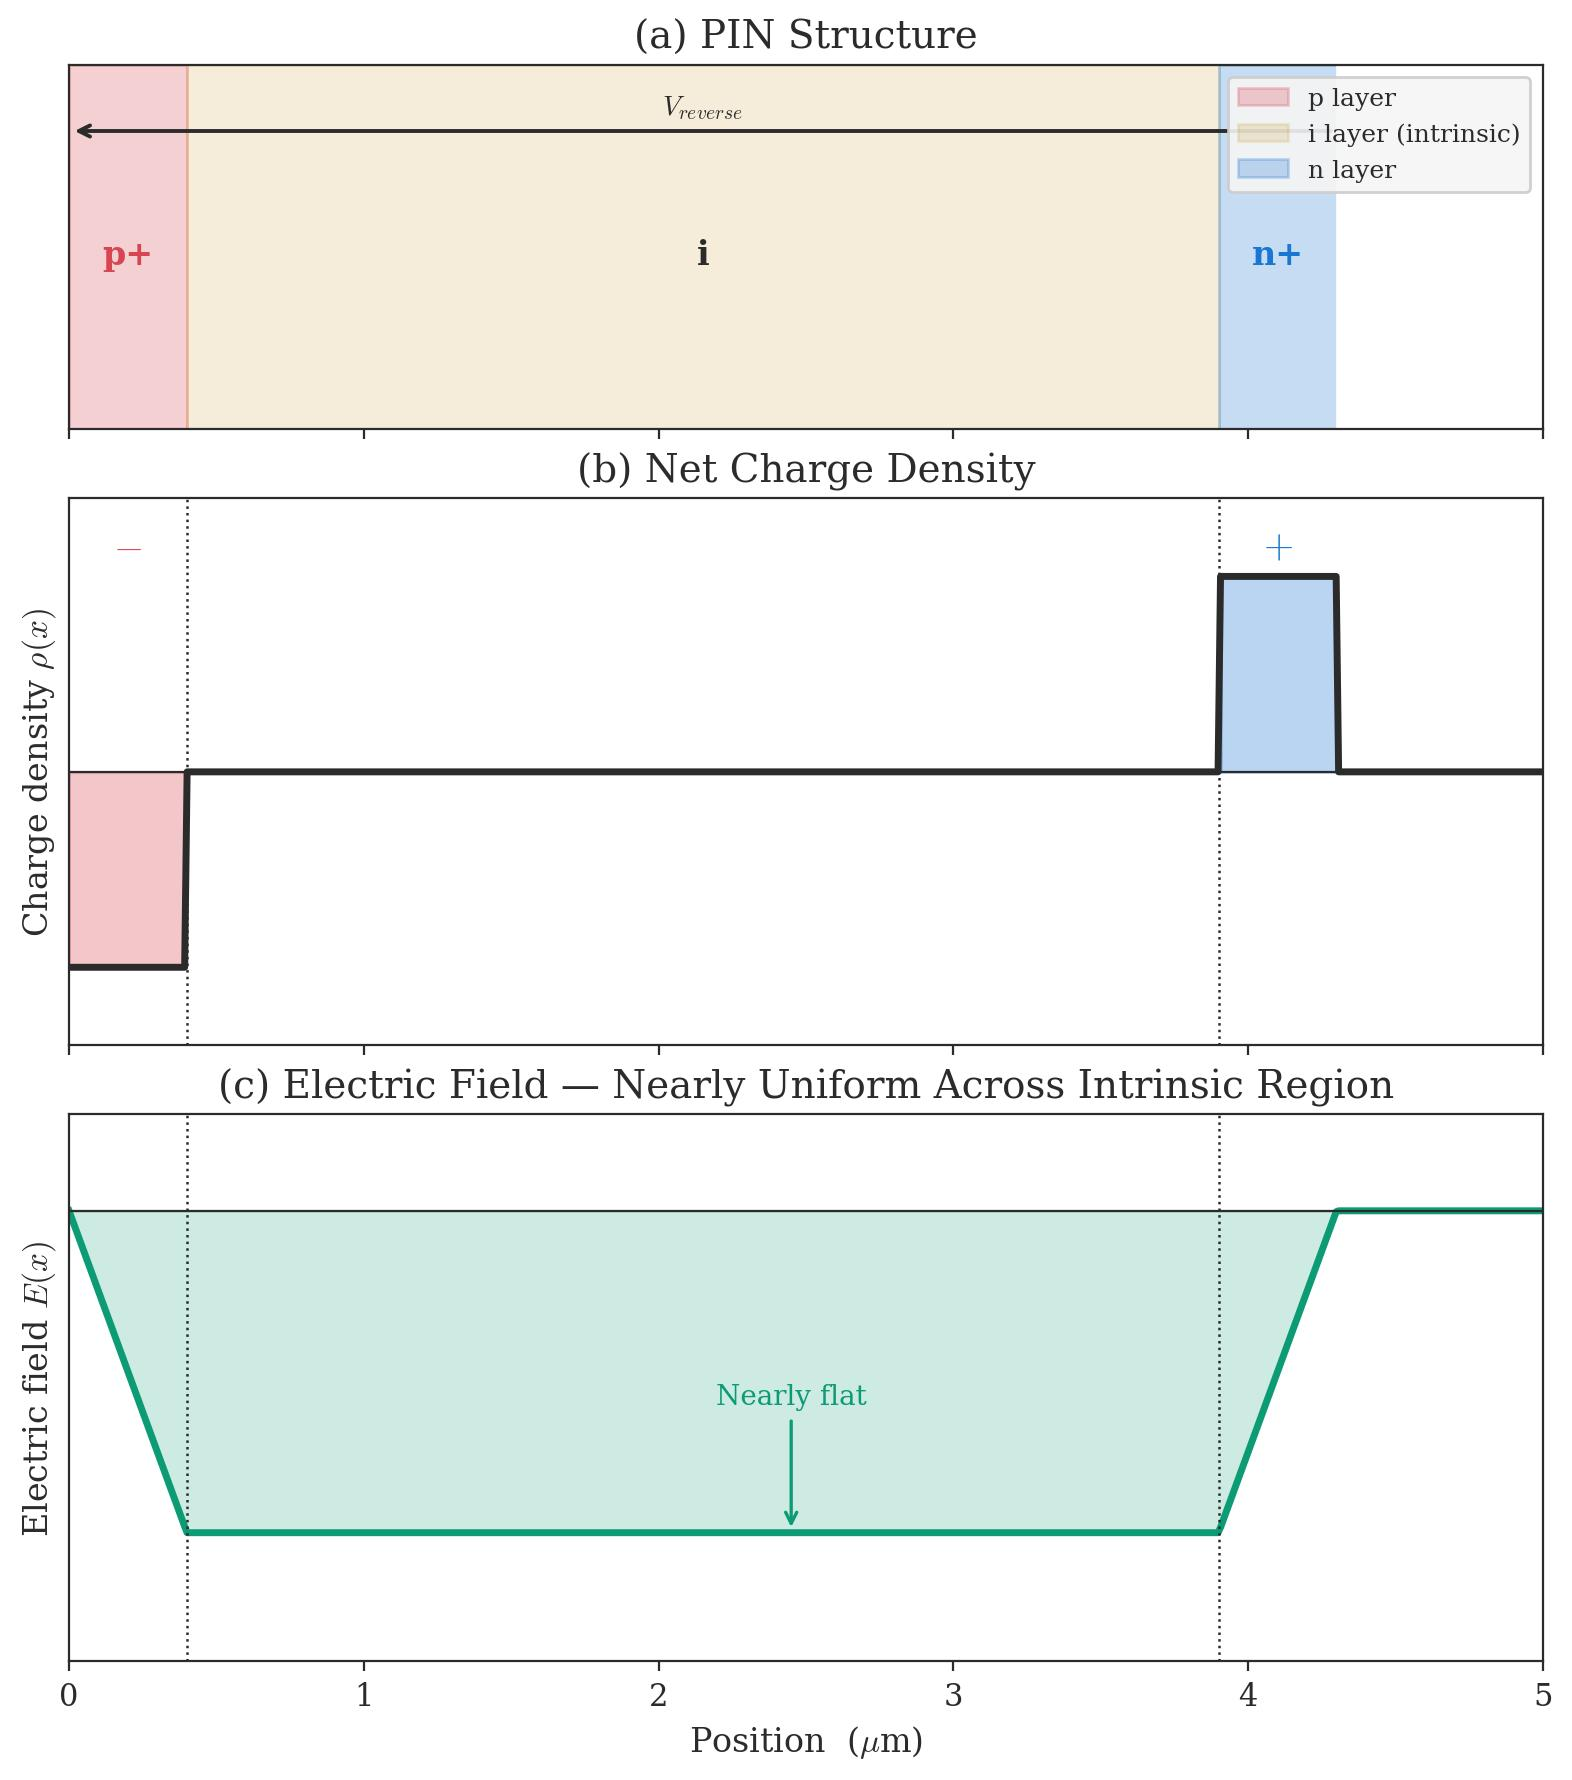
\includegraphics[width=0.7\textwidth]{Figures/Chapter 10/pin_structure_and_field.jpg}
    \caption{PIN Photodiode Structure, Charge, and Electric Field}
    \label{fig:pin_structure_and_field}
\end{figure}

\textbf{Thicker absorption region:} By making the intrinsic layer as thick as required (typically $1$--$10\,\mu$m), we can choose $\alpha W_i \gg 1$ independently of the doping — something impossible in a PN diode where the depletion width is fixed by $W_0 \propto \sqrt{V_0}$.

\textbf{Uniform electric field:} The intrinsic region contains almost no ionised dopants, so the net charge density is near zero throughout. Poisson's equation then gives a nearly flat electric field across the entire intrinsic layer — all photogenerated carriers experience the same, maximum field and are swept out at the same saturated drift velocity.

\textbf{Lower capacitance:} The junction capacitance is $C_j = \epsilon_s A / W_i$. A thicker intrinsic layer reduces $C_j$, which lowers the RC time constant and improves bandwidth.

\textbf{The trade-off:} Making $W_i$ too thick increases the carrier transit time $\tau_\text{drift} = W_i/v_d$ and ultimately limits bandwidth despite the lower capacitance. There is an optimal intrinsic layer thickness that balances these competing effects.

\subsection{Heterojunction PIN: Separating Absorption from Incidence}

A heterojunction PIN replaces the top (illuminated) layer with a wider-bandgap material. Since the wide-gap layer does not absorb photons below its bandgap, the incident light passes through it without loss and is absorbed only in the narrow-gap intrinsic region. This eliminates the surface-generated carrier problem of simple PN junctions. For InP/InGaAs receivers (the workhorse of $1.3$--$1.55\,\mu$m telecommunications), the InP window layer is transparent to the signal wavelengths while the InGaAs intrinsic region provides the efficient absorption — achieving near-ideal collection at both target wavelengths.

\begin{figure}[H]
    \centering
    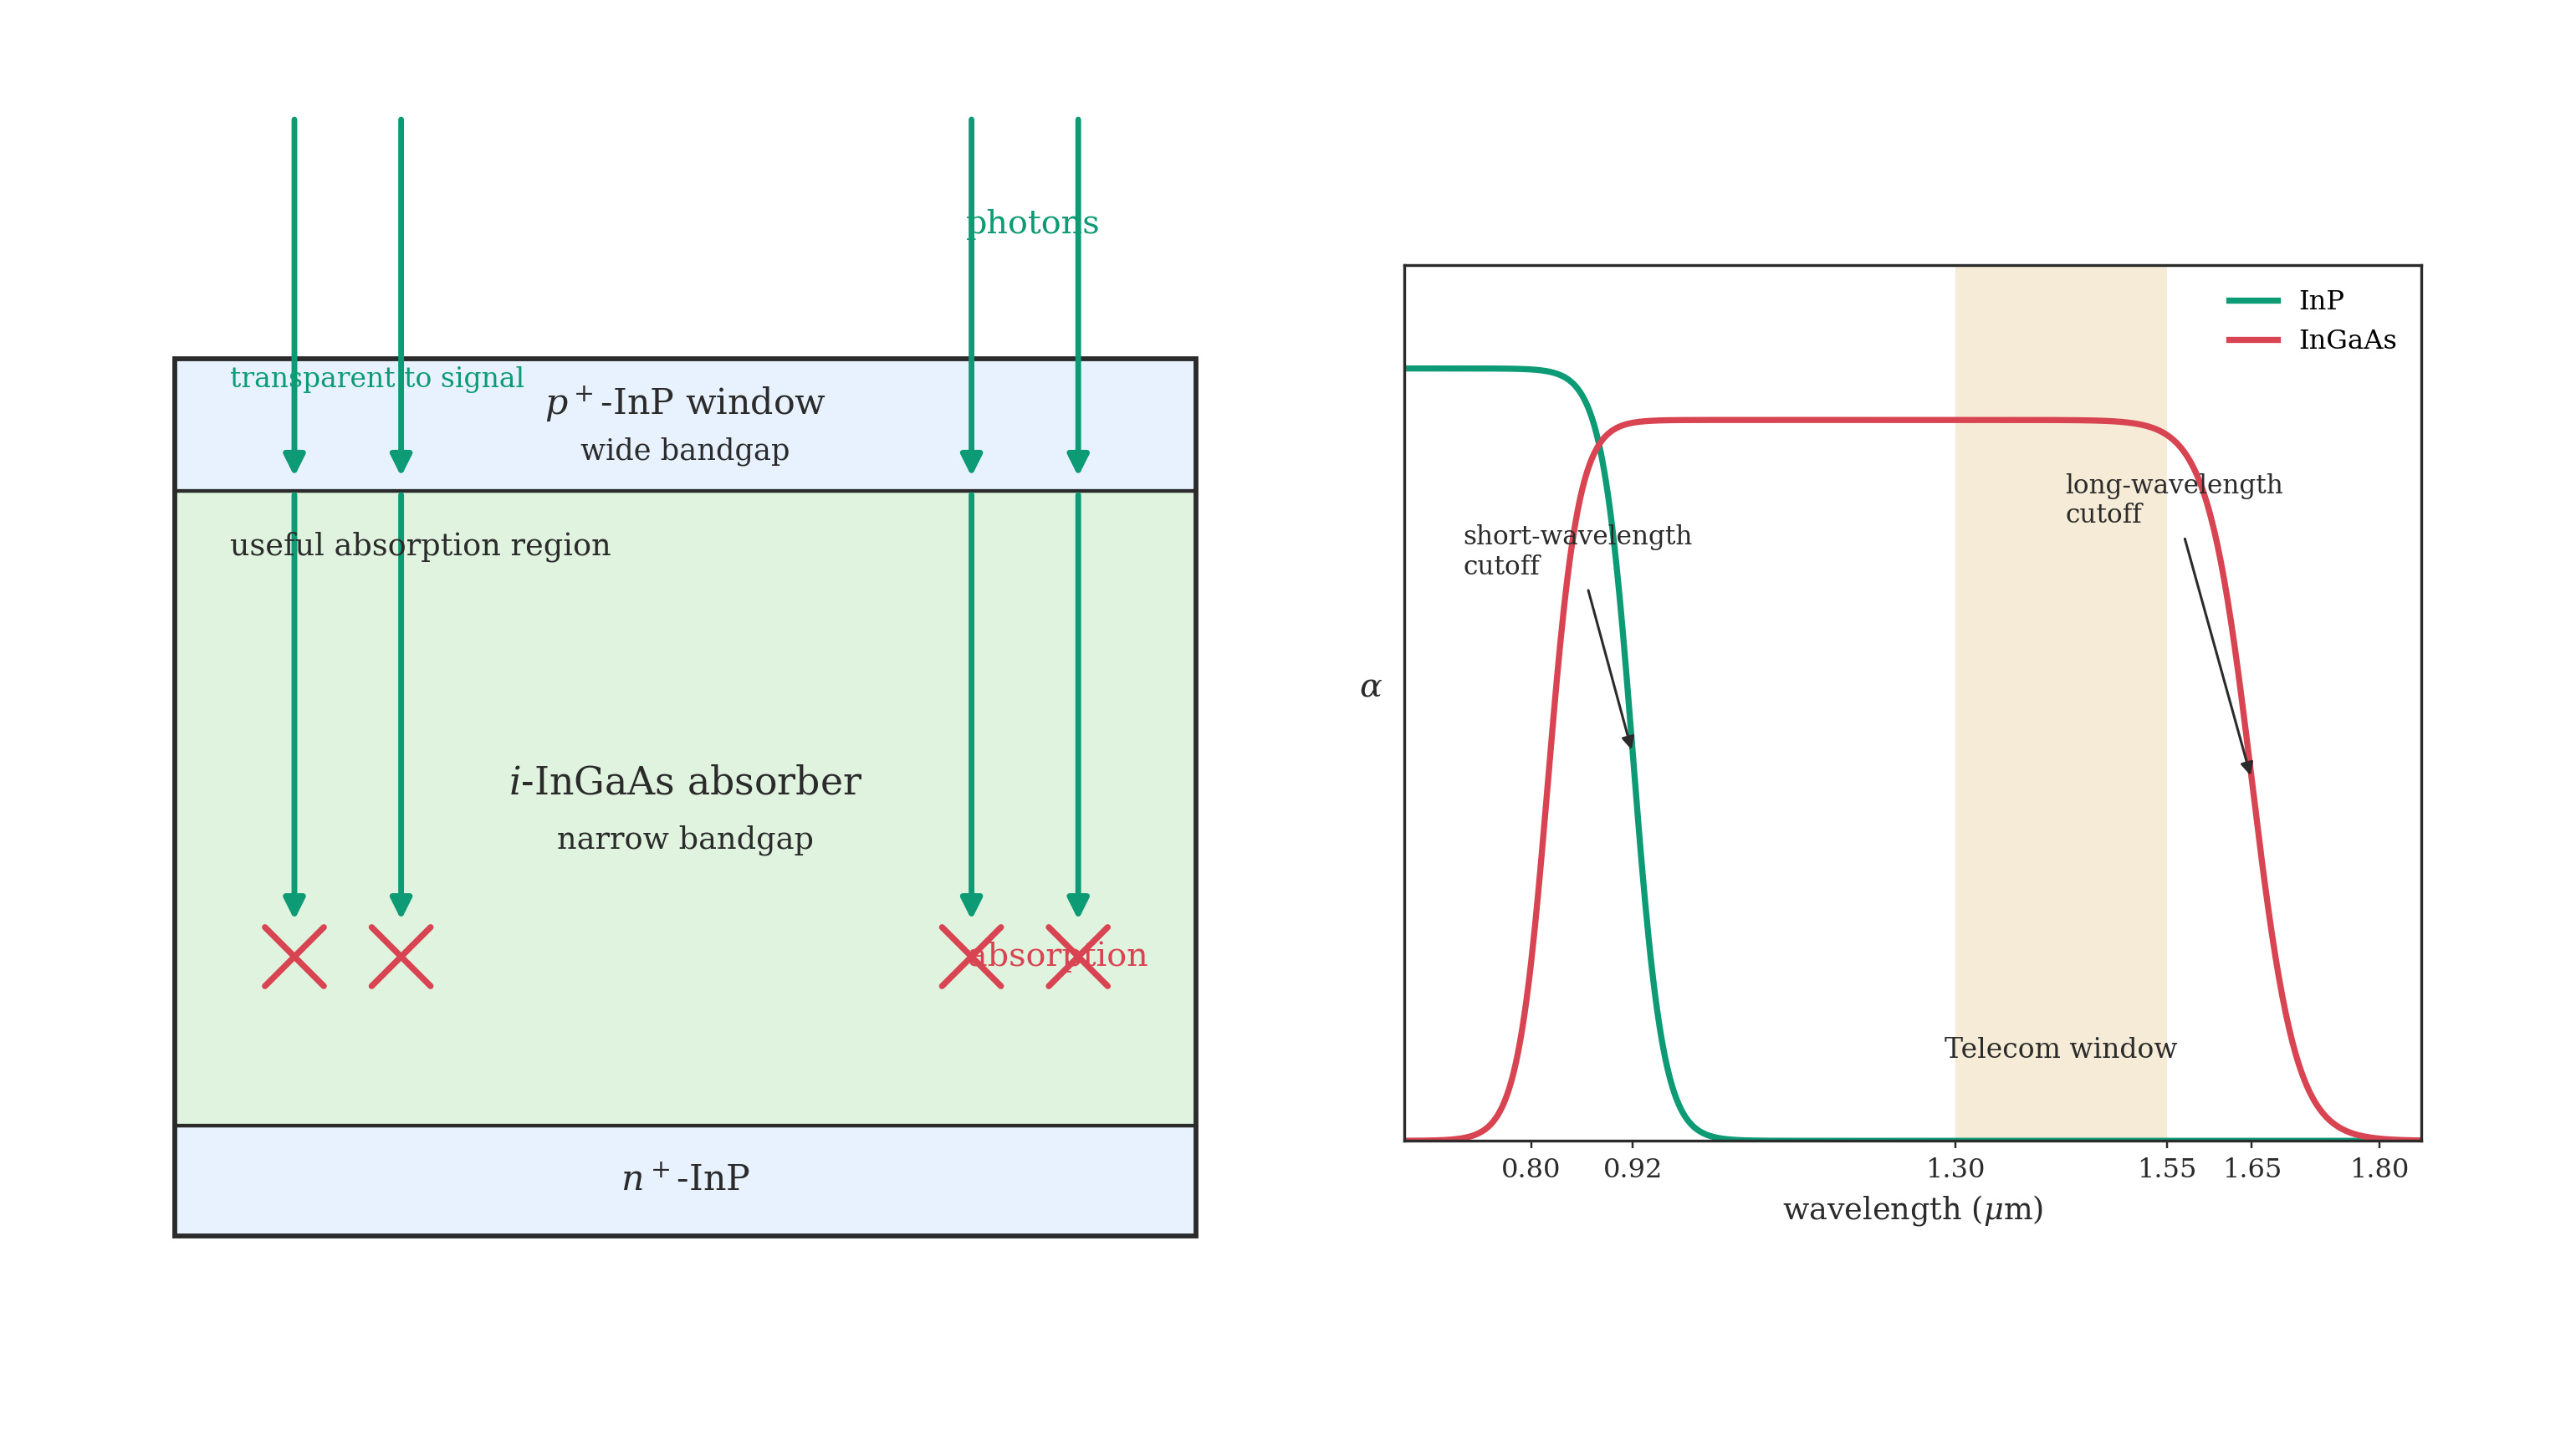
\includegraphics[width=0.7\textwidth]{Figures/Chapter 10/heterojunction_pin_photodiode_and_spectral_windowing.jpg}
    \caption{Heterojunction PIN Photodiode and Spectral Windowing}
    \label{fig:heterojunction_pin_photodiode_and_spectral_windowing}
\end{figure}

% ------------------------------------------------------------------
\section{Photocurrent and the Illuminated Diode Equation}
% ------------------------------------------------------------------

The dark current-voltage characteristic of a reverse-biased diode follows the standard Shockley equation:
\begin{equation*}
    I_D = I_s\!\left(e^{eV/k_BT} - 1\right)
\end{equation*}

Under illumination, the photogenerated current $I_p = \mathcal{R}\,P_\text{opt}$ flows in the opposite direction to the forward-bias convention (photons pull electrons from p to n, opposite to injection). The total device current is therefore:
\begin{keyresult}
    \begin{equation}
        I = I_s\!\left(e^{eV/k_BT} - 1\right) - I_p, \qquad I_p = \mathcal{R}\,P_\text{opt}
    \end{equation}
\end{keyresult}

Illumination shifts the entire $I$–$V$ curve downward by $I_p$. In the third quadrant (reverse bias, negative current), the device delivers a photocurrent $I \approx -I_p$ that is proportional to the optical power — this is the normal operating regime of a photodetector.

\subsection{Current-to-Voltage Conversion: The Sensitivity-Dynamic Range Dilemma}

The simplest readout circuit connects the photodiode in series with a load resistor $R_L$ and a bias supply $V_B$. Applying Kirchhoff's voltage law gives the load line equation:
\begin{equation*}
    V = -I R_L - V_B
\end{equation*}

The actual operating point is the intersection of this load line with the illuminated diode equation. The output voltage across $R_L$ is $V_\text{out} = I_p R_L$, which is proportional to $P_\text{opt}$ — the photodiode acts as a current source and the load resistor converts that current to a voltage.

\begin{figure}[H]
    \centering
    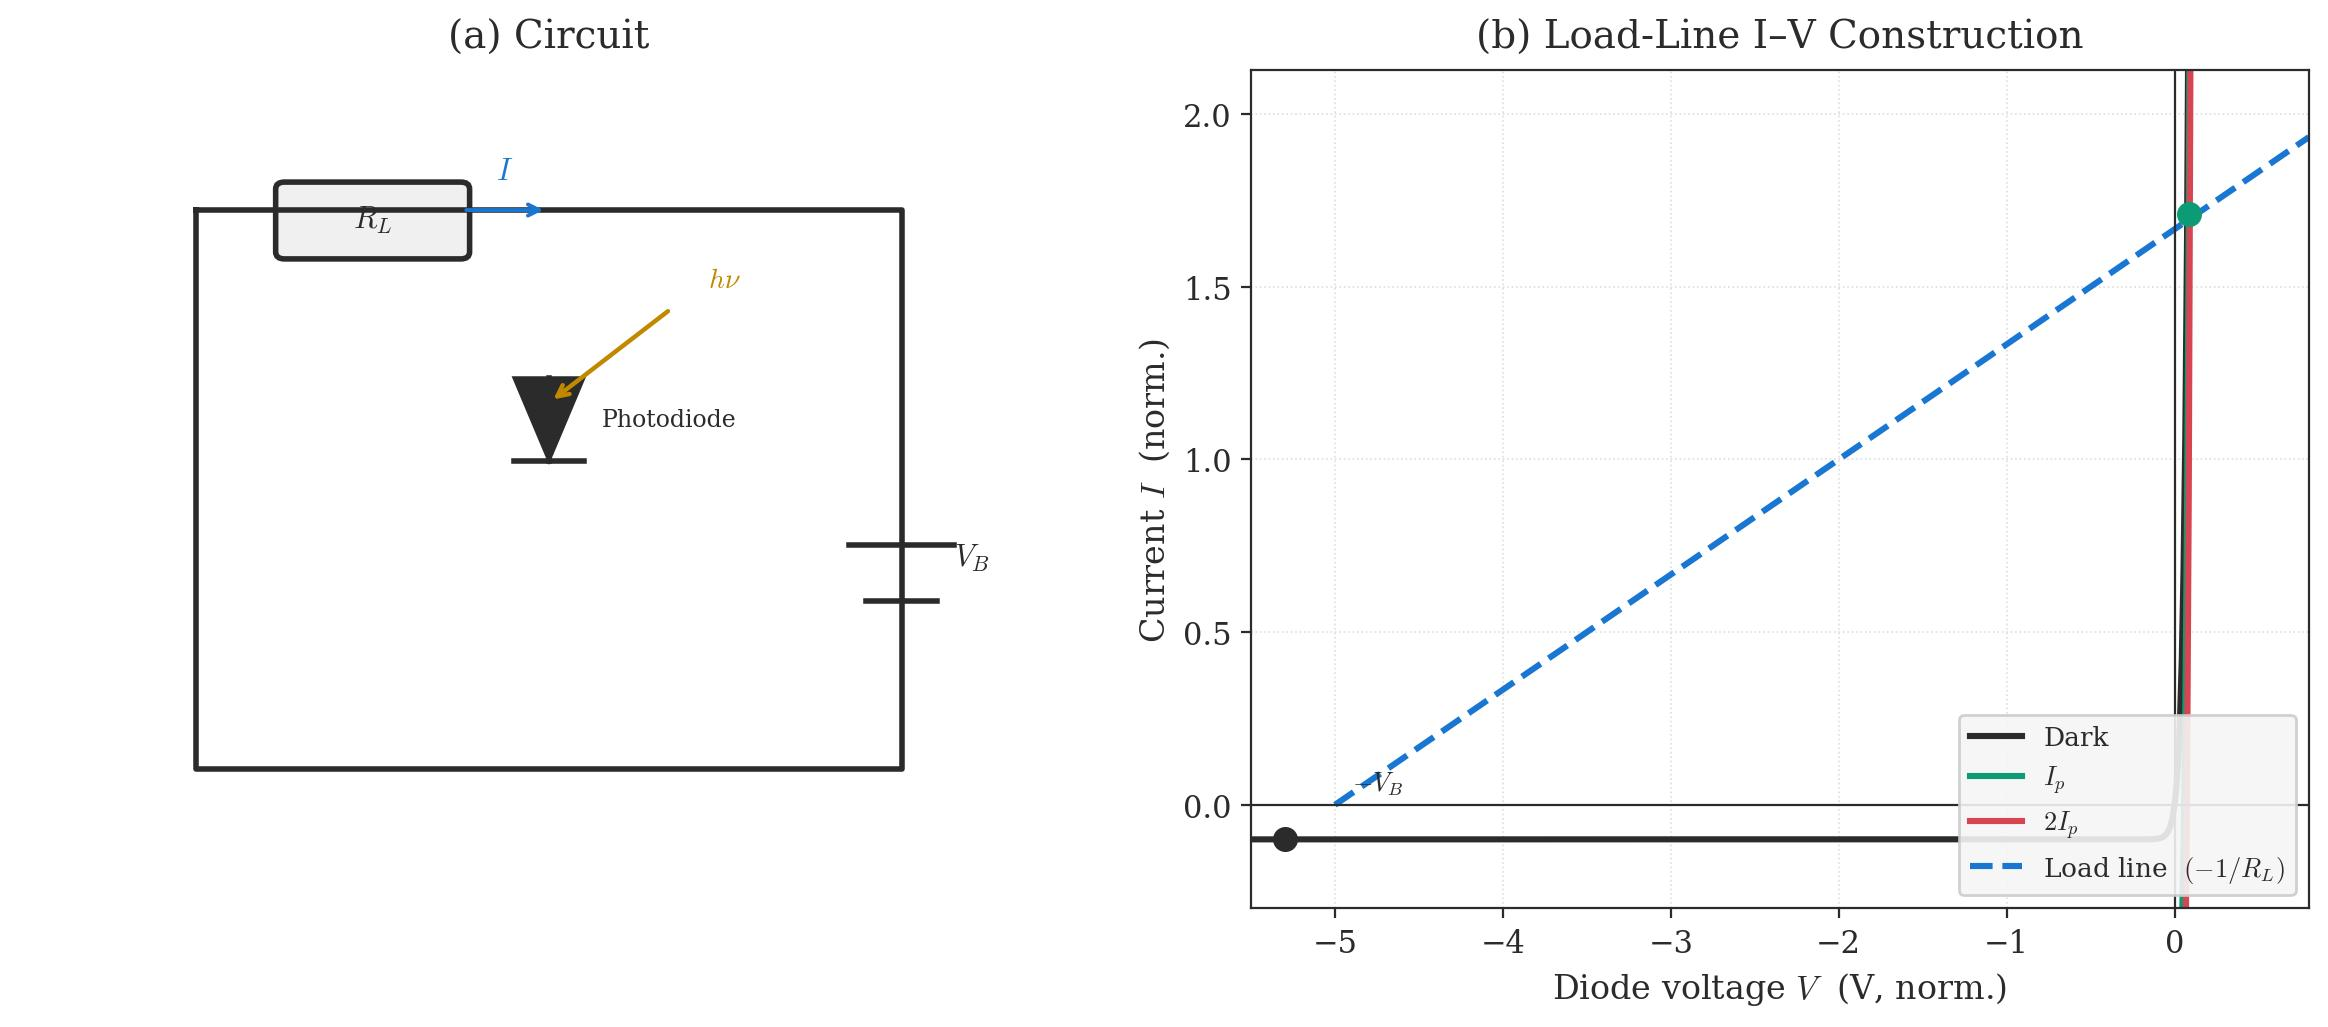
\includegraphics[width=0.6\textwidth]{Figures/Chapter 10/load_line_construction.jpg}
    \caption{Current-to-Voltage Conversion with a Load Resistor}
    \label{fig:load_line_construction}
\end{figure}

Choosing the value of $R_L$ creates a severe conflict known as the \textbf{Sensitivity-Dynamic Range Dilemma}. What is the physical mechanism here?
\begin{itemize}
    \item \textbf{Sensitivity (Low Light):} If optical power is very low, the photocurrent $I_p$ is tiny. To get a measurable output voltage $V_\text{out} = I_p R_L$, you must make $R_L$ very large.
    \item \textbf{Dynamic Range (High Light):} However, if a sudden burst of high optical power hits the detector, a large $I_p$ flows. Because $R_L$ is large, the voltage drop across it ($I_p R_L$) becomes huge. If this voltage drop equals the bias supply $V_B$, the diode voltage $V$ reaches zero (or forward bias). The electric field in the depletion region collapses, drift collection stops, and the detector violently saturates.
\end{itemize}
Therefore, a large $R_L$ gives excellent sensitivity but terrible dynamic range (and terrible bandwidth due to $\tau_{RC} = R_L C_j$). A small $R_L$ gives great dynamic range and speed, but terrible sensitivity. The simple resistor cannot win.

\subsection{The Transimpedance Amplifier (TIA)}

To break the resistor's dilemma, the simple load resistor is universally replaced by a \textbf{transimpedance amplifier} (TIA) at high data rates. A TIA uses a high-gain inverting amplifier with a feedback resistor $R_f$.

Here is a direct comparison of why the TIA completely dominates the simple resistor front-end:
\begin{itemize}
    \item \textbf{Virtual Ground (The Magic):} The amplifier actively forces the photodiode node to a virtual ground. The photodiode voltage remains rigidly clamped at a constant value regardless of the photocurrent. Because the voltage doesn't swing, the junction capacitance $C_j$ never charges or discharges, completely eliminating the $RC$ bandwidth penalty.
    \item \textbf{Independent Sensitivity:} The effective transimpedance (output voltage per input current) is set by $R_f$. We can make $R_f$ large for excellent sensitivity without collapsing the diode voltage, thus preserving huge dynamic range.
    \item \textbf{Noise Performance:} A larger $R_f$ actually \emph{improves} the signal-to-thermal-noise ratio (since signal voltage scales as $R_f$ while thermal noise voltage scales as $\sqrt{R_f}$).
    \item \textbf{The Cost (Complexity \& Power):} The price for these benefits is active power consumption, silicon area, and the requirement that the amplifier's internal gain-bandwidth product must be extremely high to maintain the virtual ground at high frequencies.
\end{itemize}

% ------------------------------------------------------------------
\section{Avalanche Photodiodes}
% ------------------------------------------------------------------

\subsection{Impact Ionisation, Microscopic Mechanics, and Avalanche Gain}

A PIN photodiode strictly converts one photon into one electron-hole pair—its absolute maximum responsivity is clamped at $\mathcal{R} = e\lambda/(hc)$. An \textbf{avalanche photodiode} (APD) breaks this ceiling by amplifying the primary photocurrent through the physical mechanism of \textbf{impact ionisation}.

What actually happens at the microscopic level?
\begin{enumerate}
    \item \textbf{Acceleration:} Under an extreme electric field (often $>10^5\,\text{V/cm}$), a photogenerated electron accelerates violently, gaining immense kinetic energy over its mean free path.
    \item \textbf{Impact:} Before it can reach the contact, the ultra-fast carrier collides directly with a stationary crystal lattice atom.
    \item \textbf{Ionisation:} If the carrier's kinetic energy is greater than the bandgap, the collision violently knocks a bound valence electron into the conduction band, freeing it.
    \item \textbf{Cascade:} One carrier has now become three (the original electron, plus the new electron and hole). These new carriers are immediately accelerated by the field in opposite directions, repeating the process over and over.
\end{enumerate}

This chain reaction—an avalanche—means that a single incident photon produces a massive burst of $M$ electrons. The total output current is $M$ times the primary photocurrent:
\begin{keyresult}
    \begin{equation}
        I = M\,I_0
    \end{equation}
\end{keyresult}

\begin{figure}[H]
    \centering
    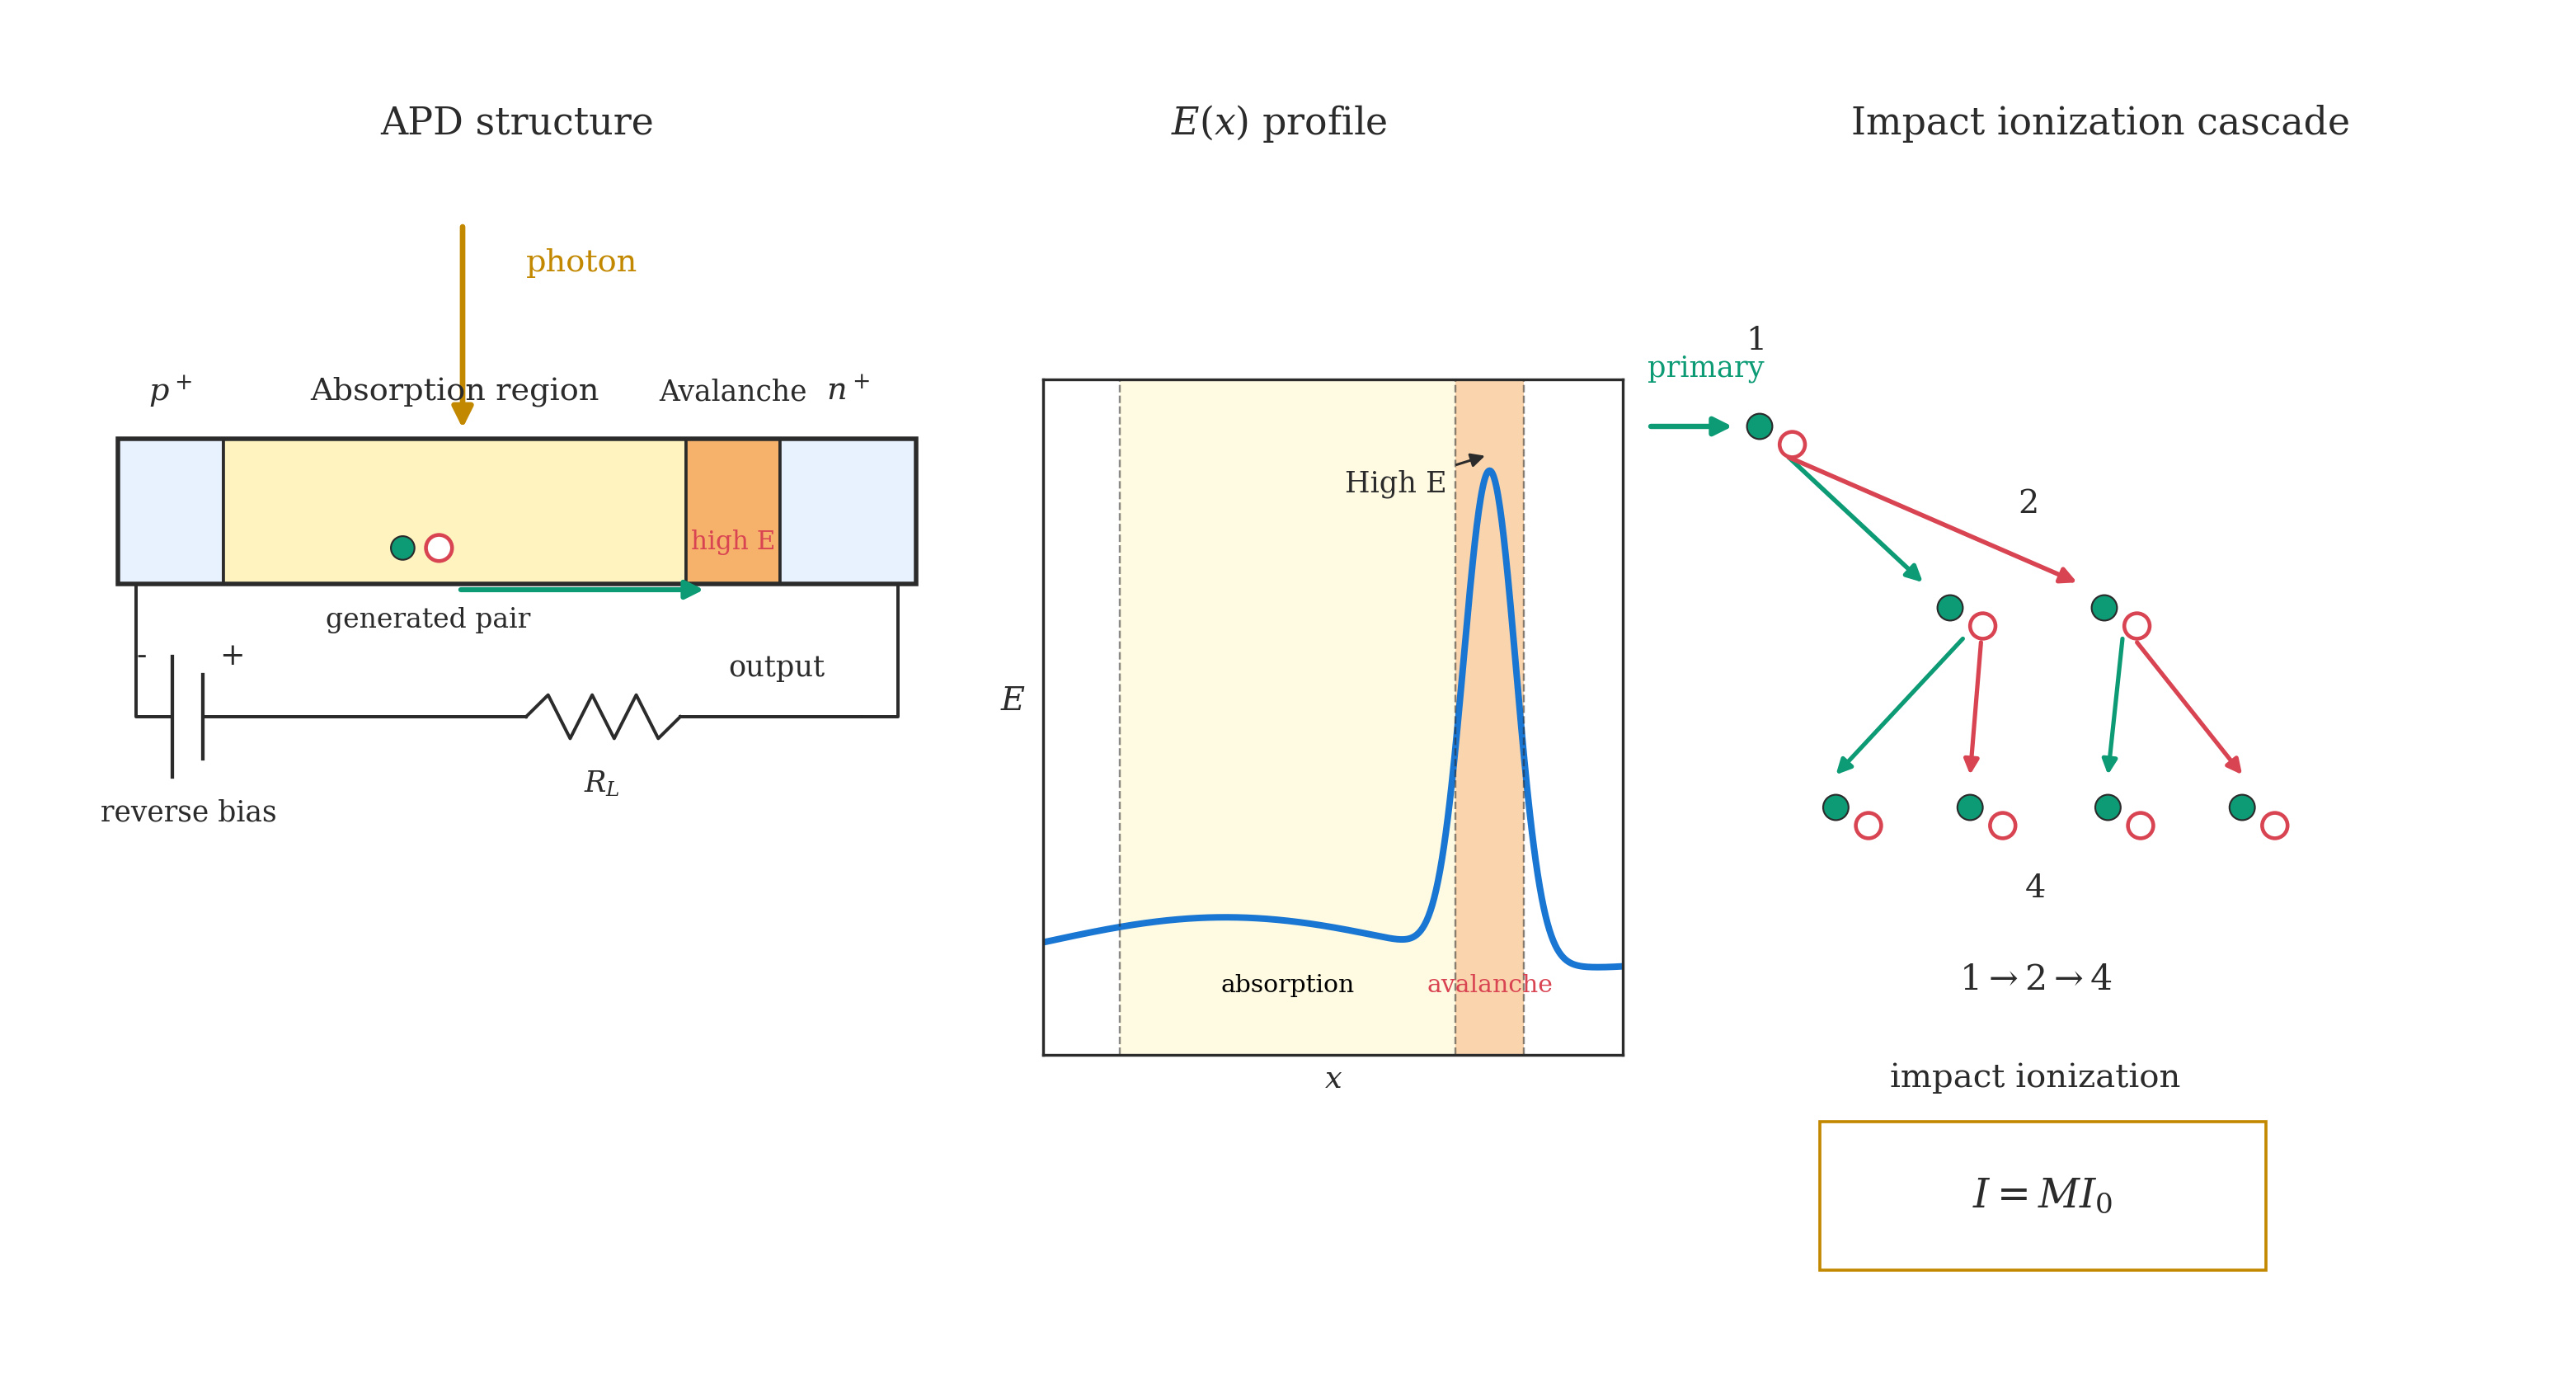
\includegraphics[width=0.7\textwidth]{Figures/Chapter 10/avalanche_photodiode_structure_and_multiplication.jpg}
    \caption{Avalanche Photodiode Structure and Multiplication}
    \label{fig:avalanche_photodiode_structure_and_multiplication}
\end{figure}

The effective responsivity is correspondingly amplified:
\begin{equation*}
    \mathcal{R}_\text{APD} = \bar{G}\,\eta\,\frac{e}{h\nu}
\end{equation*}
where $\bar{G}$ (or $M$) is the average avalanche gain. Practical values of $\bar{G} = 10$--$100$ give a monumental sensitivity advantage over PIN detectors.

\textbf{Practical Constraints (Breakdown Voltage and Temperature):}
To achieve the intense electric fields needed for impact ionisation, APDs must be biased extremely close to their reverse breakdown voltage ($V_B$). For Silicon APDs, $V_B$ typically ranges from $150\text{--}400\,\text{V}$, while Germanium APDs operate lower at $20\text{--}40\,\text{V}$.
Furthermore, the gain $M$ is wildly unstable against temperature changes. As temperature rises, the crystal lattice vibrates more intensely (more phonons). These phonons scatter the accelerating electrons, shortening their mean free path. If carriers collide too soon, they cannot accumulate enough kinetic energy to trigger ionisation, causing the gain $M$ to plummet. Thus, every practical APD requires a complex thermal-feedback circuit to actively crank up the reverse bias voltage as the device heats up, forcing the gain to stay constant.

\subsection{Cost: Excess Noise from Random Multiplication}

Avalanche multiplication is a stochastic process — not every primary carrier triggers exactly the same number of secondary ionisations. The gain fluctuates from event to event, with variance $\sigma_G^2$. This randomness adds noise beyond the fundamental shot noise of the primary photocurrent. 

To relate this variance to the average gain $\bar{G}$, we start with the definition of the gain variance:
\begin{equation*}
    \sigma_G^2 = \overline{G^2} - \bar{G}^2
\end{equation*}
Dividing both sides by the square of the mean gain $\bar{G}^2$ to normalize:
\begin{equation*}
    \frac{\sigma_G^2}{\bar{G}^2} = \frac{\overline{G^2}}{\bar{G}^2} - 1 \implies \frac{\overline{G^2}}{\bar{G}^2} = 1 + \frac{\sigma_G^2}{\bar{G}^2}
\end{equation*}
This ratio is defined as the \textbf{excess noise factor} $F$, which quantifies the noise penalty:
\begin{keyresult}
    \begin{equation}
        F = \frac{\overline{G^2}}{\bar{G}^2} = 1 + \frac{\sigma_G^2}{\bar{G}^2} \geq 1
    \end{equation}
\end{keyresult}
Since the variance $\sigma_G^2 \geq 0$, it follows that $F \geq 1$. 

To see how this affects the shot noise, consider a primary current $\bar{i}$ (such as photocurrent or dark current) composed of Poisson-distributed discrete carriers. The shot noise variance of this primary current is:
\begin{equation*}
    \sigma_\text{primary}^2 = 2e\,\bar{i}\,B
\end{equation*}
If the multiplication process were perfectly deterministic (every carrier amplified by exactly $\bar{G}$), the output noise power would scale as the square of the gain, i.e., $\sigma_\text{primary}^2 \bar{G}^2$. However, because the gain fluctuates stochastically, the total output noise is further amplified by $F$:
\begin{keyresult}
    \begin{equation}
        \sigma_\text{APD}^2 = \sigma_\text{primary}^2 \bar{G}^2 F = 2e\,\bar{i}\,B\,F\bar{G}^2
    \end{equation}
\end{keyresult}
compared to $\sigma_\text{PIN}^2 = 2Be\,\bar{i}$ for a PIN diode. The excess noise factor $F$ always exceeds 1, and it grows with increasing gain — the avalanche noise grows faster than the signal. An APD therefore provides a net sensitivity advantage only when the gain-induced signal enhancement outweighs the excess noise penalty, which occurs in the presence of significant receiver thermal noise (from $R_L$ or the TIA).

% ------------------------------------------------------------------
\section{Speed Limits and Detector Bandwidth}
% ------------------------------------------------------------------

Four distinct physical mechanisms each contribute a time delay to the detector response:

\textbf{1. Drift transit time bottleneck:} Carriers generated in the depletion region must drift across its full width $W$. Because electrons and holes have different effective masses and scattering rates, their saturation velocities are different ($v_h < v_e$). The transit times are explicitly:
\begin{equation*}
    t_e = \frac{W}{v_e} \qquad \text{and} \qquad t_h = \frac{W}{v_h}
\end{equation*}
Since the hole is the slower carrier, the transit-time bandwidth of the entire photodetector is fundamentally bottlenecked by the slower hole transit time ($t_h$).

\textbf{2. Diffusion time:} Carriers generated in the neutral regions must diffuse into the depletion region before being swept out. The diffusion time across a length $L_e$ is:
\begin{equation*}
    \tau_\text{diff} = \frac{L_e^2}{2D_c}
\end{equation*}
Diffusion is slow ($\sim$10--100$\times$ slower than drift) and is one reason why absorption in the neutral regions is undesirable — those slow carriers limit bandwidth even if they are eventually collected.

\textbf{3. RC Circuit Limit:} The photodiode behaves electrically as a photocurrent source in parallel with its junction capacitance $C_D$ and the load resistor $R_L$. The total impedance of this parallel RC network is:
\begin{equation*}
    Z(\omega) = \frac{1}{\frac{1}{R_L} + j\omega C_D} = \frac{R_L}{1 + j\omega R_L C_D}
\end{equation*}
The output voltage is $V_\text{out}(\omega) = I_p(\omega) Z(\omega)$. The electrical 3\,dB bandwidth is defined as the frequency where the power transfer function drops by half, which corresponds to the impedance magnitude dropping by $1/\sqrt{2}$ from its DC value $R_L$:
\begin{equation*}
    |Z(\omega_{3\text{dB}})| = \frac{R_L}{\sqrt{1 + (\omega_{3\text{dB}} R_L C_D)^2}} = \frac{R_L}{\sqrt{2}}
\end{equation*}
This condition is met when the imaginary term equals 1:
\begin{equation*}
    \omega_{3\text{dB}} R_L C_D = 1 \implies 2\pi f_{3\text{dB}} R_L C_D = 1 \implies f_{3\text{dB}} = \frac{1}{2\pi R_L C_D}
\end{equation*}
Substituting the parallel-plate model for the junction capacitance $C_D = \epsilon_s A / W$:
\begin{keyresult}
    \begin{equation}
        f_{3\text{dB},\text{circuit}} = \frac{1}{2\pi R_L C_D} = \frac{W}{2\pi R_L \epsilon_s A}
    \end{equation}
\end{keyresult}
Increasing $W$ helps circuit speed (lower capacitance) but hurts transit speed (longer drift distance). The optimum $W$ is where the transit time roughly equals the RC time constant.

\textbf{4. Avalanche buildup time:} For an APD, the cascade of ionisations takes a finite time to complete. The avalanche delay scales with the gain:
\begin{equation*}
    \tau_A = \frac{M\,W_A}{v_d}
\end{equation*}
where $W_A$ is the width of the high-field avalanche region. Higher gain means longer avalanche time — this is why APD gain and bandwidth are inversely linked.

Combining all four mechanisms in quadrature gives the total effective response time:
\begin{keyresult}
    \begin{equation}
        \tau_\text{eff} = \sqrt{\tau_\text{drift}^2 + \tau_\text{diff}^2 + \tau_{RC}^2 + \tau_A^2}
    \end{equation}
\end{keyresult}

\begin{figure}[H]
    \centering
    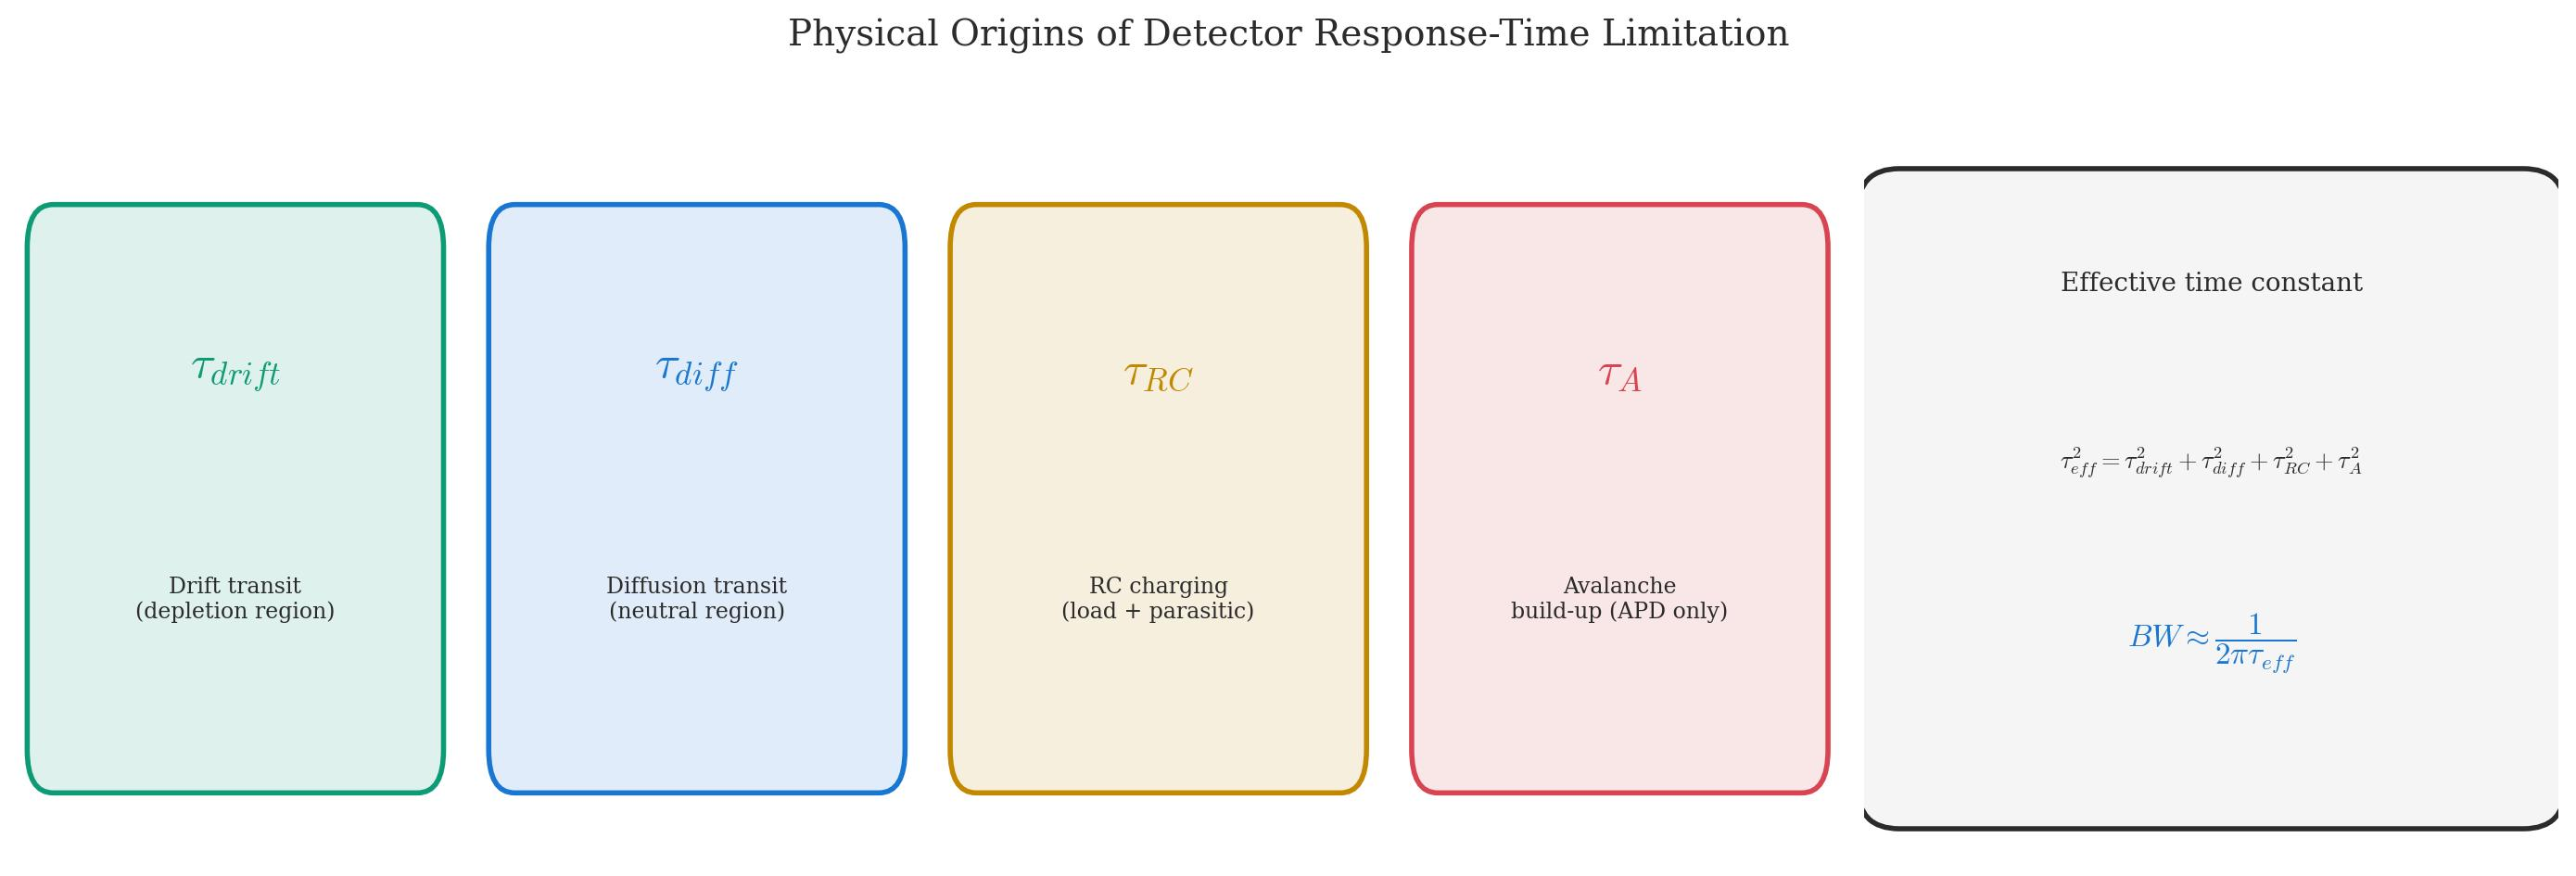
\includegraphics[width=0.7\textwidth]{Figures/Chapter 10/detector_bandwidth_contributions.jpg}
    \caption{Time-Constant Contributions to Detector Bandwidth}
    \label{fig:detector_bandwidth_contributions}
\end{figure}

The corresponding 3\,dB bandwidth is:
\begin{keyresult}
    \begin{equation}
        \text{BW} \approx \frac{1}{2\pi\,\tau_\text{eff}}
    \end{equation}
\end{keyresult}

For APDs, the avalanche buildup time imposes a \textbf{gain-bandwidth product} limit:
\begin{equation*}
    M \cdot \text{BW} \approx \frac{v_d}{2\pi\,W_A}
\end{equation*}

\begin{figure}[H]
    \centering
    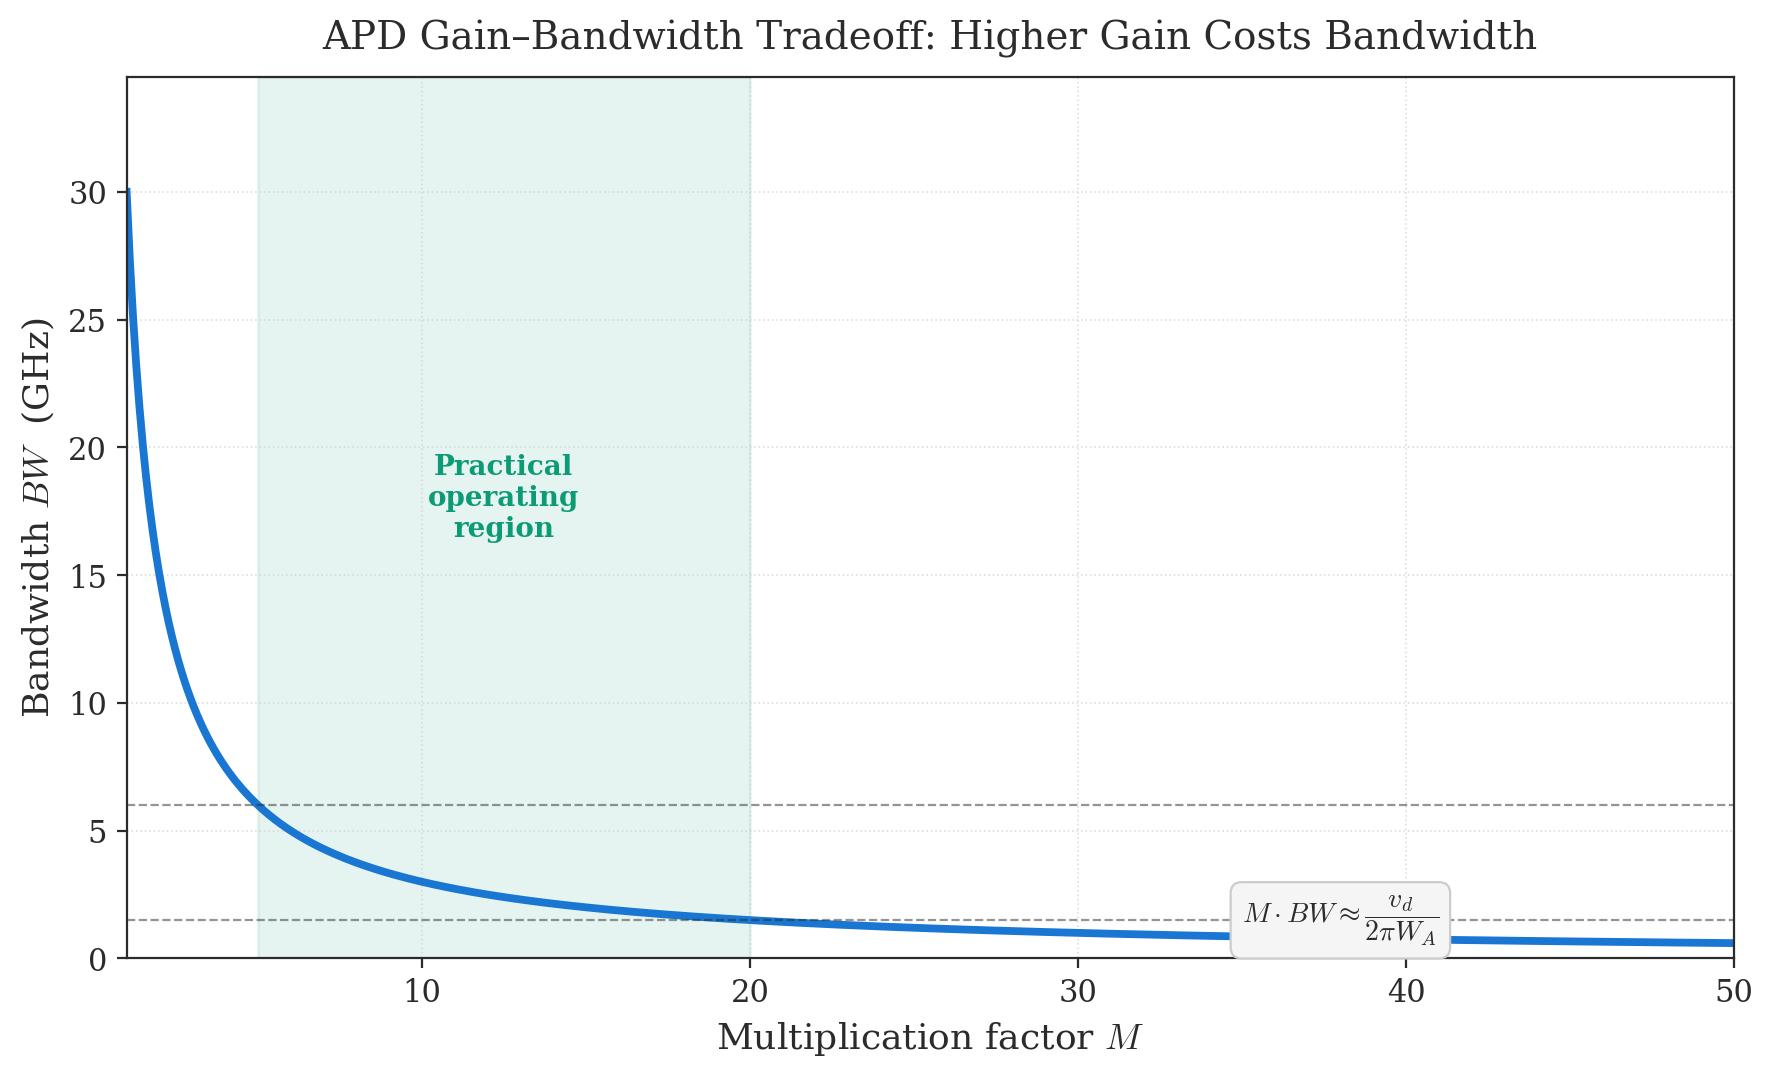
\includegraphics[width=0.6\textwidth]{Figures/Chapter 10/apd_gain_bandwidth.jpg}
    \caption{APD Gain-Bandwidth Tradeoff}
    \label{fig:apd_gain_bandwidth}
\end{figure}

This fundamental limit means that once $M$ is large enough that $\tau_A$ dominates, doubling the gain halves the bandwidth. APD design always lives at the edge of this trade-off.

% ------------------------------------------------------------------
\section{Noise in Photodetectors}
% ------------------------------------------------------------------

\subsection{Shot Noise: The Fundamental Floor and the Water Hose Analogy}

The fundamental noise mechanism in photodetection is \textbf{shot noise}—the statistical randomness in the arrival times of discrete photons and the resulting randomness in the generation of electron-hole pairs.

To gain physical intuition, imagine a \textbf{water hose} filling a bucket. If you look at the hose from far away, the water looks like a perfectly smooth, continuous stream. However, if you zoom in close to the nozzle, you realize the stream is actually made of millions of discrete, individual water droplets hitting the bucket at random intervals. Photons act exactly like those water droplets. Even if the optical power from a laser is perfectly constant on average, the photocurrent will wildly fluctuate at the microsecond level because photons arrive at random, Poisson-distributed intervals.

This droplet-like nature creates a fundamental noise current. The mean-square shot noise variance in a receiver bandwidth $B$ for a PIN photodiode is:
\begin{keyresult}
    \begin{equation}
        \sigma_\text{PIN}^2 = 2e(I_p + I_d)B
    \end{equation}
\end{keyresult}
where $I_p$ is the photocurrent and $I_d$ is the dark (reverse leakage) current of the diode. Both currents are composed of discrete charges, so both contribute to shot noise.

For an APD, the avalanche process amplifies both the signal and its shot noise, then adds additional noise from the random multiplication (quantified by the excess noise factor $F$):
\begin{keyresult}
    \begin{equation}
        \sigma_\text{APD}^2 = 2e(I_p + I_d)B \cdot F\bar{G}^2
    \end{equation}
\end{keyresult}

An important subtlety: when a photon generates one electron-hole pair, the current that flows in the external circuit is only one electron charge $e$—not $2e$. The electron and hole travel in opposite directions, but they form the two complementary halves of the same current loop. Both carriers are needed to complete the circuit, but together they deliver only $e$ of charge to the external terminal.

\subsection{Thermal (Johnson) Noise}

The load resistor $R_L$ also contributes thermal noise — random voltage fluctuations due to the thermal motion of electrons in the resistor. The mean-square Johnson noise current in bandwidth $B$ is:
\begin{equation*}
    \sigma_\text{thermal}^2 = \frac{4k_BT\,B}{R_L}
\end{equation*}

At high data rates where $R_L$ must be small to achieve the required bandwidth, thermal noise often dominates over shot noise. This is precisely the regime where APDs offer the most benefit: the internal avalanche gain boosts the signal-level shot noise above the thermal noise floor, improving the effective SNR. As $R_L$ increases (higher sensitivity designs), thermal noise diminishes relative to shot noise, and APDs provide less incremental advantage.

\subsection{Signal-to-Noise Ratio}

The received electrical SNR is the ratio of the signal power (proportional to the square of the average photocurrent) to the total noise power (the sum of shot and thermal noise variances):
\begin{equation*}
    \text{SNR} = \frac{I_\text{signal}^2}{\sigma_\text{shot}^2 + \sigma_\text{thermal}^2}
\end{equation*}

For a PIN photodiode, substituting the shot noise and Johnson thermal noise expressions:
\begin{equation*}
    \text{SNR}_\text{PIN} = \frac{I_p^2}{2e(I_p + I_d)B + \frac{4k_B T B}{R_L}}
\end{equation*}
At high data rates where $R_L$ is small, the thermal noise in the denominator typically dominates over the shot noise ($4k_B T/R_L \gg 2e(I_p + I_d)$). Applying this approximation and substituting $I_p = \mathcal{R} P_\text{opt}$:
\begin{keyresult}
    \begin{equation}
        \text{SNR}_\text{PIN} \approx \frac{(\mathcal{R}\,P_\text{opt})^2}{4k_BT B/R_L} = \frac{(\mathcal{R}\,P_\text{opt})^2 R_L}{4k_BT B}
    \end{equation}
\end{keyresult}

For an APD receiver, both the photocurrent and dark current are amplified by the average gain $\bar{G}$, and the shot noise is amplified by $\bar{G}^2 F$. Neglecting $I_d$ for simplicity, the SNR is:
\begin{equation*}
    \text{SNR}_\text{APD} = \frac{(\bar{G} I_p)^2}{2e I_p B \cdot F\bar{G}^2 + \frac{4k_B T B}{R_L}}
\end{equation*}
Substituting $I_p = \mathcal{R} P_\text{opt}$ gives:
\begin{keyresult}
    \begin{equation}
        \text{SNR}_\text{APD} \approx \frac{(\bar{G}\,\mathcal{R}\,P_\text{opt})^2}{2Be(\mathcal{R}\,P_\text{opt})\,F\bar{G}^2 + 4k_BTB/R_L}
    \end{equation}
\end{keyresult}
Note that the shot noise term in the denominator scales correctly as $\bar{G}^2$, rather than $\bar{G}^3$ which would result from incorrectly multiplying the already-amplified photocurrent by $\bar{G}^2 F$.

Optimising the APD gain $\bar{G}$ to maximise SNR for a given operating condition gives the optimal gain point — beyond which additional multiplication adds more noise than signal benefit.

\subsection{Receiver Performance Metrics: Absolute Sensitivity}

While SNR is useful for system engineers designing a specific link, device physicists need intrinsic figures of merit to compare the raw sensitivity of different detector materials independent of incident optical power or circuit bandwidth.

To do this, we systematically build a set of normalized noise metrics:

\textbf{1. Total RMS Noise Current ($I_{N\text{-RMS}}$):} First, we sum the variances of all fundamental noise sources (shot noise and thermal noise) and take the square root to find the total Root-Mean-Square noise fluctuation:
\begin{equation*}
    I_{N\text{-RMS}} = \sqrt{2e(I_p + I_d)B + \frac{4k_B T}{R_L}B} \quad [\text{A}]
\end{equation*}
where $I_d$ is the dark current (which always flows and adds shot noise).

\textbf{2. Noise Current Density ($i_{nd}$):} Because $I_{N\text{-RMS}}$ depends on the chosen bandwidth $B$, we normalize it to a $1\text{ Hz}$ bandwidth to find the intrinsic noise current density:
\begin{equation*}
    i_{nd} = \frac{I_{N\text{-RMS}}}{\sqrt{B}} = \sqrt{2e(I_p + I_d) + \frac{4k_B T}{R_L}} \quad \left[\frac{\text{A}}{\sqrt{\text{Hz}}}\right]
\end{equation*}

\textbf{3. Noise Equivalent Power ($NEP$):} The Noise Equivalent Power is the incident optical power $P_\text{opt}$ that yields an electrical signal-to-noise ratio of exactly 1. Setting $\text{SNR} = 1$ in the thermal-and-leakage noise limit (where $I_p \approx 0$ at the detection threshold):
\begin{equation*}
    \text{SNR} = \frac{I_p^2}{I_{N\text{-RMS}}^2} = \frac{(\mathcal{R} P_\text{opt})^2}{i_{nd}^2 B} = 1 \implies P_\text{opt} = \frac{i_{nd}\sqrt{B}}{\mathcal{R}} \equiv NEP(B)
\end{equation*}
This represents the bandwidth-dependent minimum detectable power. To find the intrinsic noise floor per unit bandwidth, we define the \textbf{Noise Equivalent Power Density} $NEP_{\text{den}}$ by setting $B = 1\,\text{Hz}$:
\begin{keyresult}
    \begin{equation}
        NEP_{\text{den}} = \frac{i_{nd}}{\mathcal{R}} \quad \left[\frac{\text{W}}{\sqrt{\text{Hz}}}\right]
    \end{equation}
\end{keyresult}
Any optical signal weaker than the $NEP_{\text{den}}$ is hopelessly buried in the noise floor. A smaller NEP represents a more sensitive detector.

\textbf{4. Specific Detectivity ($D^*$):} Because $NEP$ inherently scales with the physical area $A$ of the detector, comparing detectors of different sizes is unfair. Specifically, the dark leakage current is proportional to the junction area, $I_d = J_d A$, where $J_d$ is the dark current density. In leakage-dominated detectors:
\begin{equation*}
    i_{nd} \approx \sqrt{2e I_d} = \sqrt{2e J_d A} \propto \sqrt{A}
\end{equation*}
This means $NEP_{\text{den}} = i_{nd}/\mathcal{R}$ increases (worsens) proportionally to $\sqrt{A}$. To eliminate this size dependency and enable fair comparison of materials, we define the \textbf{specific detectivity} $D^*$ (pronounced "D-star") by multiplying the inverse of $NEP_{\text{den}}$ by $\sqrt{A}$:
\begin{keyresult}
    \begin{equation}
        D^* = \frac{\sqrt{A}}{NEP_{\text{den}}} = \frac{\mathcal{R}\sqrt{A}}{i_{nd}} \quad \left[\frac{\text{cm}\cdot\sqrt{\text{Hz}}}{\text{W}}\right]
    \end{equation}
\end{keyresult}
The unit is often expressed in \textbf{Jones}. A larger $D^*$ indicates a fundamentally superior detector material and architectural design, completely independent of its physical dimensions.

% ------------------------------------------------------------------
\section{Closing the Circle: What We Have Built}
% ------------------------------------------------------------------

We began this course with the simplest possible model of light-matter interaction — a single classical electron bound to a nucleus, oscillating in response to an electromagnetic wave. From that humble starting point, we have assembled the complete theoretical and practical framework of modern optoelectronics.

\begin{keyinsight}[The Intellectual Arc of This Course]
    The ten chapters of these notes form a single, unbroken chain of physical reasoning:

    \textbf{Chapters 1--2} established the microscopic language of light-matter interaction: the classical electron oscillator and its lineshape, followed by Einstein's rate equation model that introduced the quantum of light and the possibility of stimulated emission.

    \textbf{Chapter 3} showed how stimulated emission, combined with population inversion, produces \emph{optical amplification} — the travelling-wave amplifier and gain saturation. Spontaneous emission emerged as the irreducible noise floor.

    \textbf{Chapter 4} closed the loop with optical feedback: the Fabry-Pérot cavity, the oscillation threshold, mode selection, and the laser oscillator. The FP amplifier connected the sub-threshold and above-threshold regimes continuously.

    \textbf{Chapters 5--6} rebuilt the gain medium from scratch using semiconductor physics: energy bands, density of states, Fermi-Dirac statistics, quasi-Fermi levels, and the Bernard-Duraffourg gain condition. The homojunction, the double heterostructure, and the optical confinement factor $\Gamma$ emerged as the solutions to the practical problem of achieving inversion at room temperature with reasonable currents.

    \textbf{Chapters 7--8} completed the device picture: material systems (AlGaAs, InGaAsP), three recombination mechanisms, the carrier rate equation, the LED, the SOA, and the full laser diode with its P--I characteristic and temperature dependence.

    \textbf{Chapter 9} revealed the dynamics: relaxation oscillations, modulation bandwidth, turn-on delay, and the transition from multi-mode Fabry-Pérot to single-frequency DFB and DBR architectures.

    \textbf{Chapter 10 (this chapter)} completed the receiver side: optical absorption, quantum efficiency, responsivity, PIN and APD photodetectors, bandwidth limits, and noise — closing the full transmitter-channel-receiver chain of an optical communications system.

    The remarkable fact is that every step in this chain followed inevitably from the previous one. The Kramers-Kronig causality relation that ties refractive index to the absorption spectrum — first encountered in the context of atomic dispersion — reappeared when explaining why the narrow-gap active layer in a DH laser automatically has a higher refractive index than its cladding, making it a waveguide by design rather than by accident. The gain saturation formula derived for the travelling-wave amplifier resurfaced as carrier clamping in the laser diode: above threshold, the photon field collapses any excess inversion back to the threshold value, exactly as the saturation intensity did in the homogeneously broadened amplifier. The photon lifetime, first defined as the decay rate of the passive cavity, reappeared as the denominator of the relaxation oscillation frequency and as the parameter connecting threshold gain to threshold current density. This is not coincidence — it is the deep internal consistency of electrodynamics applied to matter at different scales and in different regimes.
\end{keyinsight}

Modern optoelectronics extends well beyond the scope of these lectures — quantum well and quantum dot lasers exploit confinement in two and three dimensions for even lower thresholds and higher differential gain; vertical-cavity surface-emitting lasers (VCSELs) replace cleaved facets with epitaxial Bragg mirrors to enable two-dimensional arrays; silicon photonics integrates optical and electronic functions on a CMOS platform; and quantum key distribution uses single-photon sources and detectors to implement provably secure communications. But every one of these technologies rests on exactly the physical foundations laid in these ten chapters. The tools are in hand.
